% !TEX root = omar-thesis-proposal.tex
\newcommand{\atlam}{@$\lambda$}

% Generic
\newcommand{\bindin}[2]{#1;~#2}
\newcommand{\pipe}{~\text{\large $\vert$}~}
\newcommand{\splat}[3]{#1_{#2};\ldots;#1_{#3}}
\newcommand{\splatC}[3]{#1_{#2}~~~~\cdots~~~~#1_{#3}}
\newcommand{\splatTwo}[4]{#1_{#3}#2_{#3},~\ldots~, #1_{#4}#2_{#4}}
\newcommand{\substn}[2]{[#1]#2}
\newcommand{\subst}[3]{\substn{#1/#2}{#3}}
\newcommand{\entails}[2]{#1 \vdash #2}

% Programs
\newcommand{\progsort}{\rho}
\newcommand{\pfam}[2]{\bindin{#1}{#2}}
\newcommand{\pdef}[4]{\bindin{{\sf def}~\tvar{#1}:#2=#3}{#4}}

% Families
\newcommand{\fvar}[1]{\textsc{#1}}

\newcommand{\family}[6]{{\sf tycon}~\fvar{#1}~{\sf of}~#2~\{{\sf schema~} #6; #3\}}
\newcommand{\familyDf}{\family{Tycon}{\kappaidx}{\opsort}{\opsigsort}{i}{\taurep}}

% Operators
\newcommand{\opsort}{\theta}
\newcommand{\opsigsort}{\Theta}
\newcommand{\opvar}[1]{\textbf{\textit{#1}}}

% Expressions
\newcommand{\evar}[1]{#1}
\newcommand{\efix}[3]{{\sf fix}~#1{:}#2~{\sf is}~#3}
\newcommand{\elam}[3]{\lambda #1{:}#2.#3}
\newcommand{\eapp}[2]{{#1~#2}}
\newcommand{\eopapp}[2]{\eop{Arrow}{ap}{\tunit}{#1; #2}}
\newcommand{\eop}[4]{{\fvar{#1}.\opvar{#2}\langle#3\rangle(#4)}}
\newcommand{\elet}[3]{{\sf let}~#1 = #2~{\sf in}~#3}
\newcommand{\etdef}[4]{{\sf let}~\tvar{#1} : #2 = #3~{\sf in}~#4}

% Type-Level Terms
\newcommand{\tvar}[1]{{\textbf{#1}}}

\newcommand{\tlam}[3]{\lambda \tvar{#1}{:}{#2}.#3}
\newcommand{\tapp}[2]{#1~#2}
\newcommand{\tifeq}[5]{{\sf if}~#1\equiv_{#3}#2{\sf ~then~}#4~{\sf else}~#5}
\newcommand{\tstr}[1]{\textit{``#1''}}
\newcommand{\tunit}{()}
\newcommand{\tpair}[2]{(#1, #2)}
\newcommand{\tfst}[1]{{\sf fst}(#1)}
\newcommand{\tsnd}[1]{{\sf snd}(#1)}
\newcommand{\tnil}[1]{[]_#1}
\newcommand{\tcons}[2]{#1 :: #2}
\newcommand{\tfold}[6]{{\sf fold}(#1; #2; \tvar{#3},\tvar{#4},\tvar{#5}.#6)}
\newcommand{\tinl}[2]{{\sf inl}[#1](#2)}
\newcommand{\tinr}[2]{{\sf inr}[#1](#2)}
\newcommand{\tsumcase}[5]{{\sf case}~#1~{\sf of~inl}(\tvar{#2}) \Rightarrow #3~{\sf |~inr}(\tvar{#4})\Rightarrow#5}
%\newcommand{\tsumcase}[5]{{\sf case}(#1; #2.#3; #4.#5)}
\newcommand{\tlabel}[1]{\textsl{#1}}
\newcommand{\tfamSpec}[5]{{\sf family}~[#2]~::~#3~\{#4 : #5\}}
\newcommand{\tfamSpecStd}{\tfamSpec{fam}{\kappaidx}{\taurep}{\theta}{\Theta}}

\newcommand{\ttype}[2]{\fvar{#1}\langle#2\rangle}
\newcommand{\ttypestd}{\ttype{Tycon}{\tau}}
\newcommand{\tfamcase}[5]{{\sf case}~#1~{\sf of}~\fvar{#2}\langle\tvar{#3}\rangle\Rightarrow#4~{\sf ow}~#5}
\newcommand{\trepof}[1]{{\sf repof}(#1)}

\newcommand{\tden}[2]{\llbracket #2 \leadsto #1 \rrbracket}
\newcommand{\ttypeof}[1]{{\sf typeof}(#1)}
\newcommand{\tvalof}[2]{{\sf trans}(\tden{#1}{#2})}
\newcommand{\terr}{{\sf error}}
\newcommand{\tdencase}[5]{{\sf case}~#1~{\sf of}~\tden{\tvar{#2}}{\tvar{#3}}\Rightarrow#4~{\sf ow}~#5}
\newcommand{\tderbind}[4]{{\sf let}~\tden{\tvar{#1}}{\tvar{#2}}=#3~{\sf in}~#4}

\newcommand{\titerm}[1]{\rhd(#1)}
\newcommand{\titype}[1]{{\blacktriangleright}(#1)}

\newcommand{\tconst}[1]{{\sf const}(#1)}
\newcommand{\tOp}[1]{{\sf op}(#1)}

\newcommand{\tprog}[1]{{\sf program}(#1)}

\newcommand{\topsempty}{\cdot}
\newcommand{\tops}[5]{{\sf opcon}~\opvar{#1}~{\sf of}~#2~\{#5\}}
\newcommand{\topp}[2]{#1; #2}
\newcommand{\Tops}[2]{\tvar{#1} : #2}
\newcommand{\Topp}[2]{#1; #2}
\newcommand{\kOpEmpty}{\cdot}
\newcommand{\kOpS}[2]{\opvar{#1}[#2]}
\newcommand{\kOp}[3]{#1; \kOpS{#2}{#3}}

% Tycontexts
\newcommand{\fCtx}{\Sigma}
\newcommand{\itvarCtx}{\Omega}
\newcommand{\iCtx}{\Theta}
\newcommand{\eCtx}{\Gamma}
\newcommand{\etvarCtx}{\Omega}
\newcommand{\errCtx}{\mathcal{E}}
\newcommand{\famEvalCtx}{\Xi}

% Judgments
\newcommand{\emptyctx}{\emptyset}
\newcommand{\tvarCtx}{\Delta}
\newcommand{\tvarCtxX}[2]{\Delta, {\tvar{#1}} : {#2}}
\newcommand{\fvarCtx}{\Sigma}
\newcommand{\fvarCtxX}{\Sigma, \fvarOfType{Fam}{\kappaidx}{\Theta}}
\newcommand{\eivarCtx}{\Omega}
\newcommand{\eivarCtxX}[1]{\Omega, \evar{#1}}

\newcommand{\kEntails}[3]{#1 \vdash_{#2} #3}

\newcommand{\progProg}[1]{#1}
\newcommand{\progOK}[3]{\kEntails{#1}{#2}{\progProg{#3}}}
\newcommand{\progOKX}[1]{\progOK{\tvarCtx}{\fvalCtx}{#1}}

\newcommand{\fvarOfType}[3]{\fvar{#1}[#2,#3]}
\newcommand{\fvarOfTypeDf}{\fvarOfType{Fam}{\kappaidx}{\Theta}}

\newcommand{\opOfType}[2]{#1}
\newcommand{\opType}[4]{\kEntails{#1}{#2}{\opOfType{#3}{#4}}}

\newcommand{\tOfKind}[2]{#1 : #2}
\newcommand{\tKind}[4]{\kEntails{#1}{#2}{\tOfKind{#3}{#4}}}
\newcommand{\tKindX}[2]{\tKind{\tvarCtx}{\fvalCtx}{#1}{#2}}

\newcommand{\tkindC}[4]{#1 \vdash_{#2}^\checkmark \tOfKind{#3}{#4}}

\newcommand{\isExpr}[1]{#1~\mathtt{wk}}
\newcommand{\exprOK}[3]{#1 \vdash_{#2} \isExpr{#3}}
\newcommand{\exprOKX}[1]{\exprOK{\tvarCtx}{\fvalCtx}{#1}}

\newcommand{\isIterm}[3]{#1 \vdash_#2 #3~\mathtt{wk}}
\newcommand{\isItermX}[1]{\isIterm{\tvarCtx}{\fvalCtx}{#1}}

\newcommand{\isItype}[3]{#1 \vdash_{#2} #3~\mathtt{wk}}
\newcommand{\isItypeX}[1]{\isItype{\tvarCtx}{\fvalCtx}{#1}}

\newcommand{\tEvalX}[2]{#1 \Downarrow #2}
\newcommand{\tiEvalX}[2]{#1 \curlyveedownarrow #2}

\newcommand{\fvalCtx}{\Phi}
\newcommand{\fvalCtxX}[1]{\Phi, #1}
\newcommand{\fval}[4]{\fvar{#1}\{#2; #3; #4\}}
\newcommand{\fvalDf}{\fval{Tycon}{\kappaidx}{\taurep}{\theta}}

\newcommand{\pcompiles}[3]{\vdash_{#1} #2 \Longrightarrow #3}
\newcommand{\pcompilesX}[1]{\pcompiles{\fvalCtx}{#1}{\iota}}

\newcommand{\pkcompiles}[2]{#1 \Longrightarrow #2}
%...
\newcommand{\ptcc}[2]{#1 \longrightarrow #2}

\newcommand{\etCtx}{\Gamma}
\newcommand{\etCtxX}[2]{\etCtx, \evar{#1} : #2}

\newcommand{\gtCtx}{\Psi}
\newcommand{\gtCtxX}[2]{\gtCtx, \evar{#1} \sim #2}

\newcommand{\dcheck}[6]{#1 \vdash_{#2}^{#3} #4 ~\checkmark~ #5 \leadsto #6}
\newcommand{\dcheckX}[3]{\dcheck{\Gamma}{\fvalCtx}{\Xi}{#1}{#2}{#3}}

\newcommand{\ecompiles}[5]{#1 \vdash_{#2} #3 : #4 \Longrightarrow #5}
\newcommand{\ecompilesX}[3]{\ecompiles{\etCtx}{\fvalCtx}{#1}{#2}{#3}}
\newcommand{\ecompilesA}[5]{#1 \vdash_{#2} #3 : #4 \leadsto #5}
\newcommand{\ecompilesAX}[3]{\ecompilesA{\etCtx}{\fvalCtx}{#1}{#2}{#3}}


\newcommand{\delfromtau}[4]{\vdash^{\fvar{#1}}_{#2} #3 \leadsto #4}
\newcommand{\tauisdel}[5]{\vdash^{\fvar{#1}}_{#2} \ttype{#3}{#4} \sim #5}
\newcommand{\concrep}[3]{\vdash_{#1}^{\Xi} #2 \leadsto #3}

\newcommand{\checkRC}[5]{#1 \vdash^{#2}_{#3} #4 \sim #5}
\newcommand{\checkRCX}[2]{\checkRC{\gtCtx}{\Xi}{\fvalCtx}{#1}{#2}}

\newcommand{\erase}[3]{\vdash_{#1} #2 ~\lightning~ #3}
\newcommand{\eraseX}[2]{\erase{\fvalCtx}{#1}{#2}}

\newcommand{\eCtxTogCtx}[4]{\vdash^{#1}_{#2} #3 \looparrowright #4}
\newcommand{\eCtxTogCtxX}[2]{\eCtxTogCtx{\Xi}{\fvalCtx}{#1}{#2}}

\newcommand{\ddbar}[4]{\vdash^{#1}_{#2} #3 \looparrowright #4}
\newcommand{\ddbarX}[2]{\ddbar{\Xi}{\fvalCtx}{#1}{#2}}

\newcommand{\iType}[3]{#1 \vdash #2 : #3}

\newcommand{\gtCtxH}{\hat{\gtCtx}}
\newcommand{\gtCtxHX}[2]{\gtCtxH, \evar{#1} : #2}

%
\newcommand{\fSpec}[3]{\tof{\fvar{#1}}{\kFam{#2}{#3}}}
\newcommand{\fSpecStd}{\fSpec{fam}{\kappaidx}{\Theta}}

% \tau
\newcommand{\taut}[1]{{\tau_{\text{#1}}}}
\newcommand{\tautype}{\taut{ty}}
\newcommand{\taudef}{\taut{def}}
\newcommand{\tautrans}{\taut{trans}}
\newcommand{\tauproof}{\taut{proof}}
\newcommand{\tauidx}{\taut{idx}}
\newcommand{\taui}{\taut{i}}
\newcommand{\tauidxn}[1]{\taut{idx,#1}}
\newcommand{\taurep}{\taut{rep}}
\newcommand{\taurepn}[1]{\taut{rep,#1}}
\newcommand{\tauden}{\taut{den}}
\newcommand{\tauIT}{\taut{IT}}
\newcommand{\tauarrow}{\taut{arrow}}
\newcommand{\tauprod}{\taut{prod}}
\newcommand{\tauint}{\taut{int}}
\newcommand{\taubool}{\taut{bool}}
\newcommand{\tauprog}{\taut{prog}}
\newcommand{\tauiterm}{\taut{itm}}
\newcommand{\tauval}{\taut{val}}
\newcommand{\tauop}{\taut{op}}
\newcommand{\tauD}{\taut{D}}

% \gamma
\newcommand{\ghat}{\hat{\gamma}}
\newcommand{\gabs}{\gamma_{\text{abs}}}

% \sigma
\newcommand{\delt}[1]{\sigma_{\text{#1}}}
\newcommand{\delrep}{\delt{rep}}
\newcommand{\dhat}{\hat{\sigma}}
\newcommand{\sbar}{\bar{\sigma}}
\newcommand{\sabs}{\hat{\sigma}}
\newcommand{\sabsrep}[1]{{\sf absrepof}(#1)}
\newcommand{\sconc}{\sigma_{\text{conc}}}

% \kappa
\newcommand{\kappat}[1]{\kappa_{\text{#1}}}
\newcommand{\kappaidx}{\kappat{idx}}
\newcommand{\kappai}{\kappat{i}}

% Types

% IL terms
\newcommand{\ibar}{{\bar \iota}}
\newcommand{\ivar}[1]{\textrm{#1}}
\newcommand{\ilam}[3]{\lambda #1{:}#2.#3}
\newcommand{\ifix}[3]{{\sf fix~}#1{:}#2~{\sf is}~#3}
\newcommand{\iapp}[2]{#1~#2}
\newcommand{\ipair}[2]{(#1, #2)}
\newcommand{\iunit}{()}
\newcommand{\ifst}[1]{{\sf fst}(#1)}
\newcommand{\isnd}[1]{{\sf snd}(#1)}
\newcommand{\iinl}[2]{{\sf inl}[#1](#2)}
\newcommand{\iinr}[2]{{\sf inr}[#1](#2)}
\newcommand{\icase}[5]{{\sf case}~#1~{\sf of~inl}(#2) \Rightarrow #3~{\sf |~inr}(#4)\Rightarrow#5}
\newcommand{\iintlit}{\bar{
\textrm{z}}}
\newcommand{\iop}[2]{#1 \oplus #2}
\newcommand{\iIfEq}[5]{{\sf if}~#1\equiv_{#3}#2{\sf ~then~}#4~{\sf else}~#5}
\newcommand{\mvalof}[1]{{\sf valof}(#1)}
\newcommand{\iup}[1]{{\lhd}(#1)}
\newcommand{\itransof}[1]{{\sf transof}(#1)}

% Internal Types
\newcommand{\darrow}[2]{#1\rightharpoonup#2}
\newcommand{\dint}{{\sf int}}
\newcommand{\dpair}[2]{#1\times#2}
\newcommand{\dsum}[2]{#1 + #2}
\newcommand{\dup}[1]{{\blacktriangleleft}(#1)}
\newcommand{\drepof}[1]{{\sf repof}(#1)}
\newcommand{\dunit}{\textsf{1}}



% Kinds
\newcommand{\kvar}[1]{\textrm{#1}}
\newcommand{\karrow}[2]{#1\rightarrow{#2}}
\newcommand{\kforall}[2]{\forall \kvar{#1}.#2}
\newcommand{\kstr}{\textsf{Str}}
\newcommand{\klabel}{\textsf{Lbl}}
\newcommand{\kint}{{\sf Int}}
\newcommand{\kunit}{\textsf{1}}
\newcommand{\kpair}[2]{#1 \times #2}
\newcommand{\klist}[1]{\textsf{list}[#1]}
\newcommand{\kTypeBlur}{\textsf{Ty}}
\newcommand{\kDen}{\textsf{D}}
\newcommand{\kIType}{\textsf{ITy}}
\newcommand{\kITerm}{\textsf{ITm}}
\newcommand{\ksum}[2]{#1 + #2}
% Judgements
\newcommand{\tof}[2]{#1 : #2}
\newcommand{\mtof}[2]{#1 :: #2}
\newcommand{\tentails}[2]{#1 \vdash #2}
\newcommand{\tentailst}[3]{\tentails{#1}{\tof{#2}{#3}}}
\newcommand{\tStdCtx}{\fCtx~\tvarCtx}
\newcommand{\tCtxXF}[1]{\fCtx, #1~\tvarCtx}
\newcommand{\tCtxXT}[1]{\fCtx~\tvarCtx, #1}
%\newcommand{\tCtxXL}[1]{\fCtx~\tvarCtx~\lvarCtx, #1}
\newcommand{\tentailsX}[1]{\tentails{\tStdCtx}{#1}}
\newcommand{\tentailsXt}[2]{\tentailsX{\tof{#1}{#2}}}
\newcommand{\kentails}[2]{#1 \vdash #2}
\newcommand{\kentailsX}[1]{\kentails{\fCtx}{#1}}
\newcommand{\iMkCtx}[3]{#1~#2~#3}
\newcommand{\iStdCtx}{\iMkCtx{\fCtx}{\tvarCtx}{\itvarCtx}}
\newcommand{\ientails}[2]{#1 \vdash #2}
\newcommand{\ientailsX}[1]{\entails{\iStdCtx}{#1}}
\newcommand{\casemap}[2]{#1 : #2}
\newcommand{\mentails}[3]{#1, #2 \vdash #3}
\newcommand{\mentailsX}[1]{\mentails{\tvarCtx}{\itvarCtx}{#1}}
\newcommand{\eentails}[4]{#1~#2~#3 \vdash #4}
\newcommand{\eentailsX}[1]{\eentails{\fCtx}{\tvarCtx}{\etvarCtx}{#1}}
\newcommand{\mtentails}[2]{#1 \vdash #2}
\newcommand{\mtentailsX}[1]{\mtentails{\iCtx}{#1}}
\newcommand{\mtentailsXt}[2]{\mtentails{\iCtx}{\mtof{#1}{#2}}}
\newcommand{\kSimple}[1]{#1~{\sf simple}}
\newcommand{\Tentails}[3]{#1 \vdash_{#2} #3}
\newcommand{\TentailsX}[1]{\Tentails{\fCtx}{\fvar{fam}}{#1}}
\newcommand{\kEq}[1]{#1~\mathtt{eq}}

% Verification and Translation
\newcommand{\translates}[4]{\entails{#1}{#2 \longrightarrow \tden{#3}{#4}}}

% Compilation Semantics
\newcommand{\compiless}[3]{#1 \Longrightarrow \tden{#2}{#3}}
\newcommand{\compiles}[3]{#1 \Longrightarrow \tden{#2}{#3}}
%\newcommand{\translates}[6]{\entails{#1}{\translatesTo{#2}{#3}{#4}{#5}{#6}}}
\newcommand{\translatesTo}[5]{#1 \longrightarrow \tden{#2}{\ttype{#3}{#4}{#5}{6}{7}}}
\newcommand{\translatesX}[5]{\translates{\eCtx}{#1}{#2}{#3}{#4}{#5}}

% !TEX root = omar-thesis-proposal.tex
\newcommand{\lam}[3]{\lambda #1{:}#2.#3}
\newcommand{\ap}[2]{#1~#2}
\newcommand{\z}{\textsf{z}}
\newcommand{\s}[1]{\textsf{s}(#1)}
\newcommand{\natrec}[5]{\textsf{natrec}(#1; #2; #3,#4.#5)}
\newcommand{\pair}[2]{(#1, #2)}
\newcommand{\fst}[1]{\textsf{fst}(#1)}
\newcommand{\snd}[1]{\textsf{snd}(#1)}

\newcommand{\tArrow}[2]{#1 \rightarrow #2}
\newcommand{\nat}{\texttt{nat}}
\renewcommand{\prod}[2]{#1 \times #2}

%\newcommand{\eCtx}{\Gamma}
\newcommand{\eCtxX}[3]{#1, #2 : #3}
\newcommand{\jet}[3]{#1 \vdash #2 : #3}
\newcommand{\jetX}[2]{\jet{\eCtx}{#1}{#2}}

\lstset{language=ML,
basicstyle=\ttfamily\footnotesize,
morekeywords={newcon,extends,tycon,opcon,err,schema,fix,is},
}

\section{Extending a Type System From Within}\label{att}
In this and the following two sections, we will turn our focus to language-integrated, type-oriented mechanisms for implementing extensions to the static semantics of a simply-typed programming language, to allow providers to go express finer distinctions than allowed by the general-purpose constructs (recursive labeled sums and products) that we included in Wyvern. We will return to using a fixed syntax (though as we will show, even a fixed syntax can be made quite flexible). The methods in the previous section could also be applied to the languages we will now design, but we do not integrate them explicitly because their intellectual  contributions are fundamentally orthogonal.% We will, however,  introduce a flexible dispatch mechanism for common elimination forms.
\subsection{Foundations}
Typed programming languages are often described in fragments, each consisting of a small number of indexed type constructors and associated (term-level) operator constructors. The simply typed lambda calculus (STLC), for example, consists of a single fragment containing a single type constructor, $\rightarrow$, indexed by a pair of types, and two operator constructors: $\lambda$, indexed by a type, and \verb|ap|, which we may think of as being indexed trivially. Their syntax and static semantics are shown in Fig. \ref{stlc}, written abstractly in a way that emphasizes this way of thinking about the type and term structure. A fragment is often identified by the type constructor it is organized around, so the STLC is  called $\mathcal{L}\{\rightarrow\}$, following the notational convention used by Harper \cite{pfpl} and others. 

\newcommand{\xty}[2]{\mathtt{#1}[#2]}
\newcommand{\xtyX}[1]{\xty{#1}{()}}
\newcommand{\xop}[3]{\mathtt{#1}[#2](#3)}
\newcommand{\xopX}[2]{\xop{#1}{()}{#2}}
\begin{figure}[t]
\small
\vspace{-8pt}
\begin{mathpar}
%\inferrule[var]{ }{
%	\jet{\eCtxX{\eCtx}{x}{\tau}}{x}{\tau}
%}
%
\inferrule[arrow-I]{
	\jet{\eCtxX{\eCtx}{x}{\tau}}{e}{\tau'}	
}{
	\jetX{\mathtt{lam}[\tau]({x}.e)}{\mathtt{arrow}[(\tau, \tau')]}
}

\inferrule[arrow-E]{
	\jetX{e_1}{\mathtt{arrow}[(\tau, \tau')]}\\
	\jetX{e_2}{\tau}
}{
	\jetX{\mathtt{ap}[()](e_1; e_2)}{\tau'}
}
\end{mathpar}
\vspace{-8pt}
\caption{Static semantics of the $\rightarrow$ fragment.}
\label{stlc}
\end{figure}
\begin{figure}[t]
\small
\begin{mathpar}
\inferrule[nat-i1]{ }{\jetX{\mathtt{z}[()]()}{\mathtt{nat}[()]}}

\inferrule[nat-i2]{
	\jetX{e}{\mathtt{nat}[()]}
}{
	\jetX{\xopX{s}{e}}{\xtyX{nat}}
}

\inferrule[nat-e]{
	\jetX{e_1}{\xtyX{nat}}\\
	\jetX{e_2}{\tau}\\
	\jet{\eCtxX{\eCtxX{\eCtx}{x}{\xtyX{nat}}}{y}{\tau}}{e_3}{\tau}
}{	
	\jetX{\xopX{natrec}{e_1; e_2; x, y.e_3}}{\tau}
}
\end{mathpar}
\caption{Static semantics of the $\mathtt{nat}$ fragment.}
\label{natfrag}
\end{figure}

G\"odel's $\mathbf{T}$, or  $\mathcal{L}\{\rightarrow \mathtt{nat}\}$, consists of the $\rightarrow$ fragment and the \verb|nat| fragment, defining natural numbers and a recursor that allows one to ``fold'' over a natural number. The static semantics of this fragment, also written abstractly with explicit type and operator indices, is shown in Fig. \ref{natfrag}. The language $\mathcal{L}\{\rightarrow \mathtt{nat}\}$ is  more powerful than $\mathcal{L}\{\rightarrow\}$ because the STLC admits an embedding  into  $\mathbf{T}$ but the reverse is not true. Buoyed by this fact, we might go on by adding fragments that define sums, products and various forms of inductive types (e.g. lists), or perhaps a general mechanism for defining inductive types. Each fragment also increases the expressiveness of our language by the same argument.

If we consider the $\forall$ fragment, however, defining universal quantification over types (i.e. parametric polymorphism), we must take a moment to refine our understanding of embeddings. In $\mathcal{L}\{\rightarrow\,\forall\}$, studied by Girard as System $\mathbf{F}$ \cite{girard1971extension} and Reynolds as the polymorphic lambda calculus \cite{Reynolds94anintroduction}, it is known that sums, products, and inductive and co-inductive types can all be weakly defined by a technique analagous to Church encodings. This means that we can \emph{translate} well-typed terms of a language like $\mathcal{L}\{\rightarrow\forall~\mathtt{nat} + \times\}$ to well-typed terms in $\mathcal{L}\{\rightarrow\forall\}$ in a manner that preserves their dynamic semantics. But Reynolds, in a remark that recalls the ``Turing tarpit'' of Perlis \cite{Perl82a}, reminds us that discarding the source language and programming directly with the corresponding \emph{embedding} may be unwise \cite{Reynolds94anintroduction}: 
\begin{quote}
To say that any reasonable function can be expressed by some program is not to say that it can be expressed by the most reasonable program. It is clear that the language requires a novel programming style. Moreover, it is likely that certain important functions cannot be expressed by their most efficient algorithms.
\end{quote}

%Adding new fragments directly to a language can make statically reasoning about programs more precise, support a more natural programming style and endow the language with a more favorable cost semantics. The latter two points might be relevant even if a strong embedding (i.e. one where there is a semantics-preserving isomorphism between terms and types of the fragment and the language) can be found. 
%
%Consistent with this view, typed programming languages like ML expose, for example, both $n$-ary product types and record types, despite the fact that any product type is definable using a record type (or in the other direction, using a module to provide the field selection operator). The compiler, on the other hand, \emph{is} mainly concerned with implementing the dynamic semantics correctly, and indeed, compilers often use the fact that weak definability results are quite readily derivable to their advantage, translating the constructs of an external language (EL) to those of a much simpler internal language (IL), e.g. with only binary products, during or directly after typechecking\todo{cite Harper-Stone}. %Correctly implementing the dynamic semantics of the language becomes the primary concern during this phase, so a simple IL that decreases the number of cases needing consideration when implementing and verifying the compiler is a wise choice.

%Having established why a minimal language like $\mathcal{L}\{\rightarrow\forall\}$, while suitable as an internal language, needs to be extended with additional fragments before it is suitable for use as a human-facing external language, 
An \emph{isomorphic embedding} of a typed language fragment, i.e. one that preserves static reasoning principles, in a sense that we will make more precise as we go on, can be far more difficult to establish than a weak embedding. For example, the aforementioned embedding of $\mathcal{L}\{{\rightarrow}~{\forall}~\mathtt{nat}~{+}~{\times}\}$ into $\mathcal{L}\{\rightarrow\forall\}$ does not preserve type disequality and some other equational reasoning principles (we will see less subtle issues with more complex fragments soon). Establishing an isomorphic embedding that is also natural, as measured to a first approximation, by the amount of boilerplate code that must be manually generated (and how likely one is to make a mistake when writing it), and that has a reasonable cost semantics is harder still. But these are the criteria one must satisfy to claim that a new language is unnecessary, because an embedding is satisfactory.

Modern general-purpose languages do, of course, provide constructs, like datatypes, records and abstract types, that admit strong and often satisfying embeddings of many language fragments, occupying what their designers and users see as ``sweet spots'' in the design space. However, ``general-purpose'' and ''all-purpose'' remain quite distinct, and situations continue to arise in both research and practice where desirable fragments can still only be weakly defined in terms of general-purpose constructs, or an isomorphic embedding, while possible, is widely seen as too verbose, brittle or inefficient:

\begin{enumerate}
%\compresslist
\item General-purpose constructs continue to evolve. There are many  variants of product types: records, records with functional record update, labeled tuples (records that specify a field ordering, unlike records) and record-like data structures with field delegation (of various sorts). Similarly, sum types also admit many variants (e.g. various forms of open sums). These are  either awkward or impossible to isomorphically embed into general-purpose languages that do not support them. Even something as seemingly simple as a type-safe \verb|sprintf| operator requires special support from languages like Ocaml.
\item Perhaps more interestingly, specialized type systems that enforce stronger invariants than general-purpose constructs are capable of enforcing are often developed by researchers. One need take only a brief  excursion through the literature to discover language extensions that support data parallel programming \cite{chakravarty2007data}, concurrency \cite{reppy1993concurrent}, distributed programming \cite{Murphy:2007:TDP:1793574.1793585}, dataflow programming \cite{mandel2005reactiveml}, authenticated data structures \cite{Miller:2014:ADS:2535838.2535851}, database queries \cite{Ohori:2011:MSM:2034773.2034815},  units of measure \cite{conf/cefp/Kennedy09} and many others.% All of these are implemented as dialects of existing languages, presumably because a strong encoding was not feasible.
\item Safe and natural foreign function interfaces (FFIs) require enforcing the type system of the foreign language within the calling language. %Using  a FFI that does not do this can lead to safety issues, even when both languages are separately known to be safe. 
%Safe FFIs generally require direct extensions to the language. 
For example, MLj extended Standard ML with constructs for safely and naturally interfacing with Java \cite{benton1999interlanguage}. For any other language, including  others on the JVM like Scala and the many languages that might be accessible via a native FFI, there is no way to guarantee that language-specific invariants are statically maintained, and the interface is far from natural.
\end{enumerate}

These sorts of innovations are generally disseminated as distinct \emph{dialects} of an existing general-purpose language, constructed either as a fork, using tools like compiler generators, DSL frame\-works or  language workbenches, or directly within a particular compiler for the language, sometimes activated by a flag or pragma. This, as we have argued, is quite unsatisfying: a programmer can choose either a dialect supporting an innovative approach to parallel programming or one that builds in support for statically reasoning about units of measure, but there may not be an available dialect supporting both. Forming such a dialect is alarmingly non-trivial, even in the rare situation where a common framework has been used or the dialects are implemented within the same compiler, as these mechanisms do not guarantee that different combinations of individually sound dialects remain sound when combined. Metatheoretic and compiler correctness results can only be derived for the dialect \emph{resulting} from a language   composition operation, so in a sufficiently diverse software ecosystem, dialect providers have little choice but to leave this task to clients (providing, perhaps, some informal guidelines or partial automation). Avoiding dialect composition is difficult, because interactions between components of an application written in different dialects can lead to precisely the problems of item 3.% We will consider this further in our discussion of related work in Sec. \ref{related-work}.

These are not the sorts of problems usually faced by library providers. Well-designed languages preclude the  possibility of ``link-time'' conflicts between libraries and ensure that the semantics of one library  cannot be weakened by another by strictly enforcing abstraction barriers. For example, a module declaring an abstract type in ML can rely on its representation invariants no matter which other modules are in use, so clients can assume that they will operate robustly in combination without needing to attend to burdensome ``link-time'' proof obligations. 

----

We begin in Sec. \ref{atlam} by developing a core calculus called @$\lambda$ and focusing on theoretical issues, including type safety, decidability and {conservativity} (that extensions cannot weaken one another, in any combination). We will also sketch a flexible type-directed dispatch mechanism for standard syntactic forms that targets this core calculus, relying fundamentally on the idea of associating extension logic with types. We then give examples of simple but interesting extensions that are built into, or are only weakly definable, in modern functional languages. 

This provides a bridge to allow us to continue on in Sec. \ref{ace} with the task of designing and implementing a full-scale programming language based on similar mechanisms called Ace. We will show more interesting examples of statically-typed general-purpose abstractions, as well as specialized abstractions (including the entirety of the OpenCL programming language for GPU programming), implemented as libraries in Ace. Ace  uses Python as its type-level language and supports user-defined base and target languages, rather than picking a fixed base language ($\mathcal{L}\{\rightarrow\}$) and target language ($\mathcal{L}\{\rightharpoonup \kint~\kunit \times{+}\}$) as in @$\lambda$. Ace also supports an extensible form of ``just-in-time'' staging: dynamic class tags extracted from Python values can propagate into the Ace compiler as static types at the point during execution where an Ace function is called from a Python script. We show that this is particularly well-suited for scientific workflows.% characterized by periods of exploratory programming punctuated by computations that demand more performance, stronger correctness guarantees or specialized abstractions. 

Ace is aimed squarely at achieving the goal of \emph{expressiveness}. That is, it helps advance the goal of this work, which is to give programmers orthogonal access to a richer variety of features from within a single   language. Python is at one extreme, initially providing effectively only a single type, \texttt{dyn}, so it poses an interesting challenge. Using a type-level language that provides few strictly enforced semantic guarantees makes giving strong metatheoretic guarantees about Ace more difficult. Ace does include checks similar to those in @$\lambda$ that catch most accidental problems but they can be intentionally subverted by untrusted extension providers using the dynamic metaprogramming features of Python. We conjecture, but do not plan to show in this thesis, that it would be possible to use Ace to bootstrap a statically-typed subset of Python that, if used to compile extension logic, would be sufficient to provide theoretical guarantees comparable to @$\lambda$ (building, perhaps, on recent work that resulted in a mechanized semantics for Python \cite{pysem}).

%But, as mentioned in Section \ref{language-integrated-approaches}, some significant challenges must be addressed before such a mechanism can be relied upon. The desire for expressiveness must be balanced against  concerns about maintaining various safety properties in the presence of arbitrary combinations of user-defined  extensions to the language's core semantics. The mechanism must ensure that desirable \emph{metatheoretic properties} (e.g. type safety, decidability) of the language are maintained by extensions. Because multiple independently developed extensions might be used within one program, the mechanism must further guarantee that extensions are \emph{conservative}. These are the issues we seek to address in the next two sections.

\section{@$\lambda$}\label{atlam}
%Programming languages are typically organized around a monolithic collection of indexed type and operator constructors. Let us begin by considering the simply-typed lambda calculus (STLC). It provides a single type constructor, indexed by a pair of types, that we will call $\fvar{Arrow}$ for uniformity. It also provides two operator constructors: $\lambda$, indexed by a type, and $\texttt{ap}$, indexed trivially. We can specify the static semantics of the STLC as follows, using a uniform abstract syntax where type and operator indices are written in braces to emphasize this way of thinking about its structure:
%
%Although a researcher may casually speak of ``conservatively extending the STLC`` with a primitive natural number type and its corresponding operators (as in G\"odel's T; Figure \ref{nat-statics}) or primitive product types and their  corresponding operators (Figure \ref{pair-statics}), it is clearly not possible to directly introduce these from within the STLC.
%\begin{figure}[h]
%\small
%\vspace{-8pt}
%\begin{mathpar}
%\inferrule[nat-I1]{ }{
%	\jetX{\texttt{z}[()]()}{\fvar{Nat}[()]}
%}
%
%\inferrule[nat-I2]{
%	\jetX{e}{\fvar{Nat}[()]}
%}{
%	\jetX{\texttt{s}[()](e)}{\fvar{Nat}[()]}
%}
%
%\inferrule[nat-E]{
%	\jetX{e_1}{\fvar{Nat}[()]}\\
%	\jetX{e_2}{\tau}\\
%	\jet{\eCtxX{\eCtxX{\eCtx}{x}{\fvar{Nat}[()]}}{y}{\tau}}{e_3}{\tau}
%}{
%	\jetX{\texttt{natrec}[()](e_1; e_2; x.y.e_3)}{\tau}
%}
%\end{mathpar}
%\vspace{-8pt}
%\caption{Static semantics of natural numbers.}\label{nat-statics}
%\vspace{-15pt}
%\end{figure}
%\begin{figure}[h]
%\small
%\begin{mathpar}
%\inferrule[Prod-I]{
%	\jetX{e_1}{\tau_1}\\
%	\jetX{e_2}{\tau_2}
%}{
%	\jetX{\texttt{pair}[()](e_1; e_2)}{\fvar{Prod}[(\tau_1, \tau_2)]}
%}
%
%\inferrule[Prod-E1]{
%	\jetX{e}{\fvar{Prod}[(\tau_1, \tau_2)]}
%}{
%	\jetX{\texttt{prl}[()](e)}{\tau_1}
%}
%
%\inferrule[Prod-E2]{
%	\jetX{e}{\fvar{Prod}[(\tau_1, \tau_2)]}
%}{
%	\jetX{\texttt{prr}[()](e)}{\tau_1}
%}
%\end{mathpar}
%\vspace{-8pt}
%\caption{Static semantics of products}\label{pair-statics}
%\end{figure}
%
%One recourse researchers have in such situations is to attempt to encode new constructs in terms of existing constructs. Collections of such encodings are sometimes called \emph{embedded domain-specific languages (EDSLs)} \cite{fowler2010domain}. Unfortunately, finding an encoding that fully captures both the static and dynamic semantics of a desirable construct can be difficult\footnote{For example, Church encodings in System F were among the more challenging topics for students in our undergraduate programming languages course, 15-312.} and is not always possible. Even when it possible, it may be impractical to work with and optimize. For our example of adding natural numbers or products to the STLC, an encoding is impossible. In closely-related languages, like the polymorphic lambda calculus (a.k.a. System F), such constructs are only weakly definable via Church encodings \cite{reynoldsIntroToPolymorphism} and far from practical. Reynolds, echoing Perlis   \cite{perlisPearl}, puts it succinctly \cite{reynoldsIntroToPolymorphism}:
%
%\begin{quote}
%To say that any reasonable function can be expressed by some program is not to say that it can be expressed by the most reasonable program. It is clear that the language requires a novel programming style.
%Moreover, it is likely that certain important functions cannot be expressed by their most
%efficient algorithms.
%\end{quote}
%

%creating a new language. If this is not practical, the best one can attempt to do is encode the new types in terms of existing types (by a Church encoding, for example). This is generally unsatisfactory -- 

%Languages implemented using these common patterns are central planning by a language designer or design committee. 

%Researchers or domain experts who cannot work around such limitations must develop new standalone languages. In our simple scenario, we may simply copy our implementation of G\"odel's T or even edit it directly (a pernicious technique for implementing a new language where the prior one is overwritten). In a more complex scenario, we may instead employ a tool like a compiler generator or DSL framework \cite{fowler2010domain} that can generate a standalone implementation from declarative specifications of language constructs. Some of these tools allow you to package and reuse these specifications (with the important caveat that not all combinations of constructs are valid and free of conflicts, an important modularity issue that we will return to several times in this paper).
%
%The increasing sophistication and ease-of-use of these tools have led many to suggest a {\it language-oriented approach} \cite{journals/stp/Ward94} to software development where different components of an application are written in different languages. Unfortunately, this leads to problems at language boundaries: a library's external interface must only use constructs that can reasonably be expressed in \emph{all possible calling languages}. This can restrict domain-specific languages by, for example, precluding constructs that rely on statically-checked invariants stronger than those their underlying representation in a common target language normally supports. At best, constructs like these can be exposed by generating a wrapper where run-time checks have been inserted to guarantee necessary invariants. This compromises both verifiability and performance and requires the development of an interoperability layer for every DSL. Moreover, library clients must work with verbose and unnatural ``glue code'' when interfacing across languages, defeating the primary purpose of high-level programming languages: hiding the low-level details from the end-users of abstractions. We diagram this fundamental \emph{compatibility problem} in Figure \ref{approaches}(a).
%\begin{figure*}
%\begin{center}
%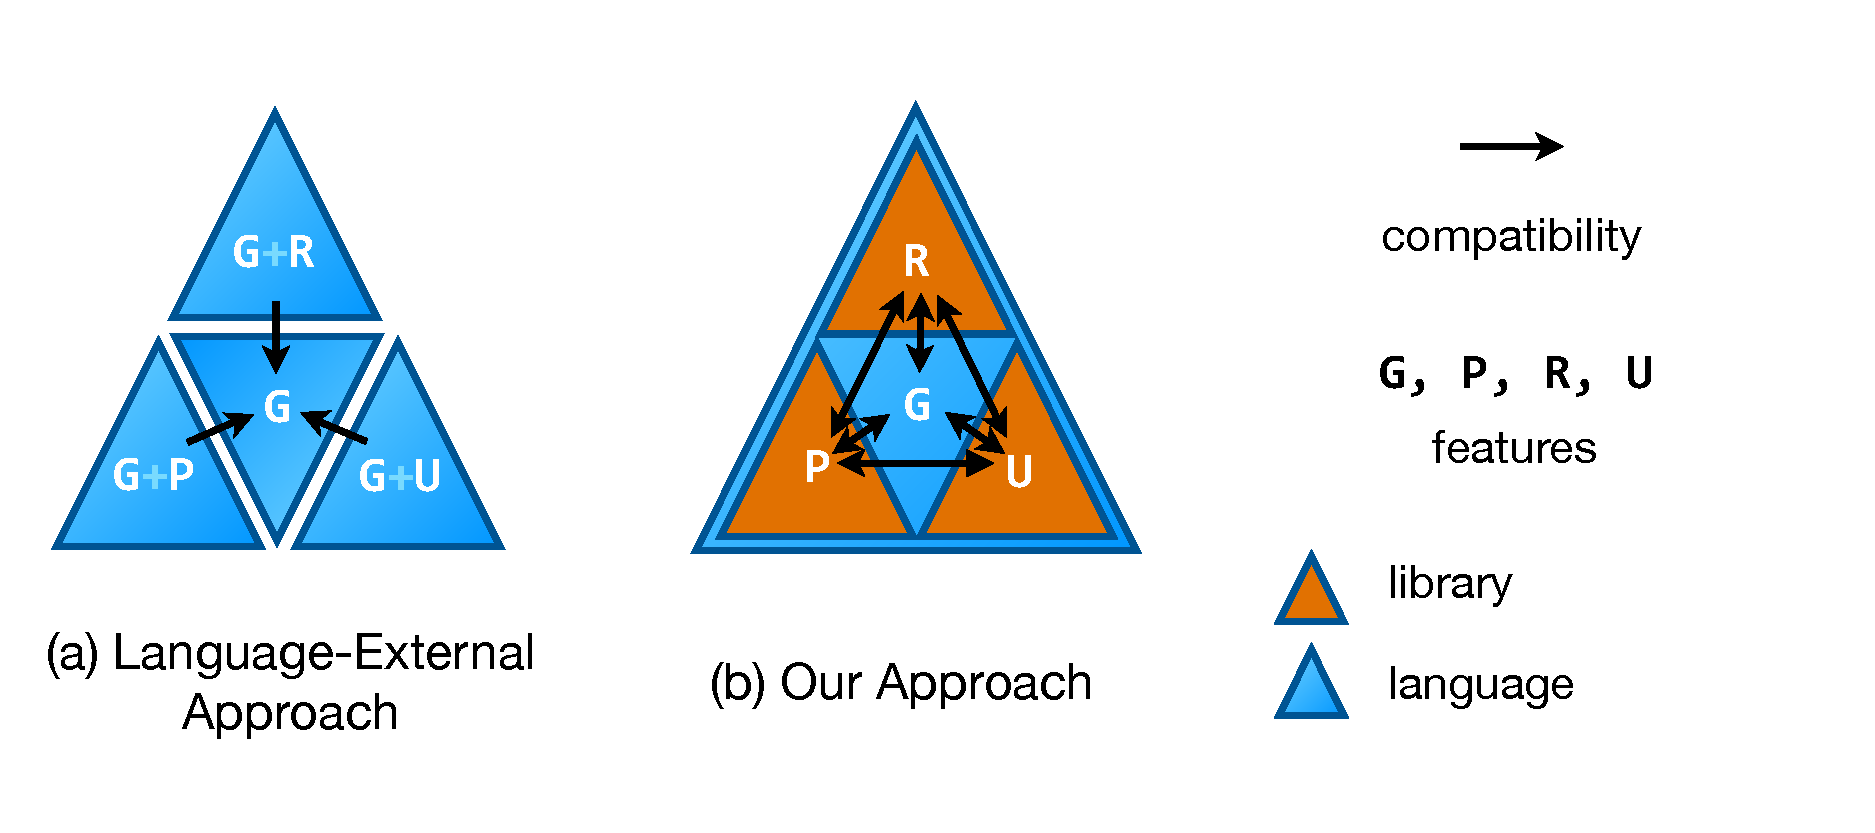
\includegraphics[scale=0.5]{approaches.pdf}
%\end{center}
%\vspace{-20px}
%\caption{\small (a) With a language-oriented approach, novel constructs are packaged into separate languages. Users can only safely and naturally call into languages consisting of common constructs (often only the common target language, such as C or Java bytecode). (b) With a language-internal extensibility approach, there is one system providing a common internal language, where additional primitive constructs that strictly strengthen its static guarantees or perform specialized code generation are specified and distributed within libraries. \label{approaches}}
%\end{figure*}

%As a result, domain-specific languages and new general-purpose abstractions alike have experienced relatively slow adoption in practice.
%
%Porting large codebases to new languages is difficult, and the dominant programming languages innovate slowly, so programming language.
%
%More specifically, such languages are neither \emph{internally extensible} because the language itself exposes only natural numbers and functions to its users, nor are they \emph{externally extensible} because no new behaviors can be added to the language's  implementation in a separate module from the one containing the initial implementation.

%This is the essence of a monolithic language implementation: it is impossible for anyone to modularly extend languages defined in this way. 

%\subsection{Theory}\label{atlam}
%%\begin{figure}
%%\begin{mathpar}
%%\inferrule{a}{b}
%%\end{mathpar}
%%\end{figure}
%In this section, we will describe a minimal calculus that captures our language-internal extensibility mechanism,  called \emph{active typechecking and translation (AT\&T)}. AT\&T allows developers to declare new primitive type families, associate operators with them, implement their static semantics in a functional style, and realize their dynamic semantics by simultaneously implementing a translation into a typed internal language. Note that this latter mechanism is closely related to how Standard ML was (re-)specified\todo{cite/read a bit about this/ask Bob/flesh this out}, but that we are fundamentally interested in extending language \emph{implementations}, not their  declarative specifications; proving the adequacy of such implementations against mechanized specifications, or extracting them directly from such specifications, will be investigated in future work.
%
%The AT\&T mechanism utilizes type-level computation of higher kind and integrates typed compilation techniques into the language to allow us to give strong metatheoretic guarantees,  and uses a mechanism notionally related to abstract types (such as those found in the ML module system) to guarantee that extensions cannot interfere with one another,  while remaining straightforward and expressive. In this section, we will develop a core calculus, called \atlam, which uses a minimal, uniform grammar for primitive operators. Then in Section \ref{ace}, we will show how to realize this minimal mechanism within a widely-used language with a more expressive grammar.
%
%AT\&T is general with respect to many choices about the type-level language, the typed internal language and syntax. Choices along these dimensions can affect both expressiveness and ease-of-use. We will begin in Sec. 2 by introducing a minimal system called $@\lambda$ (the ``actively-typed lambda calculus'') that distills the essence of the mechanism in a simply-typed, simply-kinded setting. This will allow us to fully and concisely formalize the language and compiler and give several key safety theorems. We will then continue in Sec. 3 by discussing variants of this mechanism based on other basic paradigms, considering dependently-typed functional languages and object-oriented languages, discussing trade-offs between expressivity and safety when doing so. We have developed a simple prototype called Ace and have used it to develop a number of full-scale language extensions as libraries. We will briefly discuss this language and these extensions in Sec. 4.

%We note at the outset that AT\&T focuses on extending the static semantics of languages with fixed, though flexible, syntax. Language-internal syntax extension mechanisms have been developed in the past (e.g. SugarJ \cite{sugarj}) but they have also suffered from safety problems because grammar composition is not always safe when done in an  unconstrained manner. Tyconstrained approaches that provide stronger safety guarantees have recently been outlined (e.g. Wyvern \cite{globaldsl13}) but we will leave integration of syntax extensions with semantic extensions as future work.


%\subsubsection{@$\lambda$: Conservatively Extending a Type System From Within}
\begin{figure}[t]
\small
$$\begin{array}{rccl}	
\textbf{programs} & \rho & ::= & \pfam{\familyDf}{\progsort} 
%\pipe \pdef{t}{\kappa}{\tau}{\progsort} 
\pipe e\\
		&	\theta	&	::= &	\tops{op}{\kappaidx}{i}{a}{\taut{def}} \pipe 
												\topp{\theta}{\theta}\\
\\
\textbf{external terms} 				&	e	&	::=	&	\evar{x} \pipe 
%														\efix{x}{\tau}{e} \pipe 
														\elam{\evar{x}}{\tau}{e} \pipe 
														\eop{Tycon}{op}{
															\tauidx
														}{
  												    		\splat{e}{1}{n}
														} \\
									& 		&		& 	\\


\textbf{internal terms} 				& 	\iota	&	::=	&	\evar{x} \pipe 
												\ifix{\evar{x}}{\sigma}{\iota} \pipe
												\ilam{\evar{x}}{\sigma}{\iota} \pipe 
												\iapp{\iota_{1}}{\iota_{2}} \pipe
												\iintlit \pipe \iop{\iota_{1}}{\iota_{2}} \pipe \iIfEq{\iota_{1}}{\iota_{2}}{\dint}{\iota_{3}}{\iota_{4}} \\
										& & \pipe & 
												\iunit \pipe
												\ipair{\iota_{1}}{\iota_{2}} \pipe 
												\ifst{\iota} \pipe
												\isnd{\iota} \pipe
												 \iinl{\sigma_2}{\iota_1} \pipe \iinr{\sigma_1}{\iota_2} \pipe \icase{e}{x}{e_1}{x}{e_2} \\
												
%\text{deabstracted}& \iota & ::= & \mathcal{G}[\iota, \sigma]\\
\textbf{internal types}			&	\sigma	&	::=	&    \darrow{\sigma_1}{\sigma_2} \pipe \dint \pipe \dunit \pipe \dpair{\sigma_1}{\sigma_2} \pipe \dsum{\sigma_1}{\sigma_2}  
												
\\
\\
							
\hspace{-5pt}\textbf{type-level terms} 	& \tau 	& ::= 	& 	\tvar{t} \pipe 
														\tlam{t}{\kappa}{\tau} \pipe 
														\tapp{\tau_1}{\tau_2} \pipe
														\tnil{\kappa} \pipe \tcons{\tau_1}{\tau_2} \pipe 
									                     \tfold{\tau_1}{\tau_2}{h}{t}{r}{\tau_3}
														\\
												
	 			& 		& \pipe	& 	 \iintlit \pipe \iop{\tau_1}{\tau_2} \pipe \tlabel{label} \pipe \tunit \pipe 
														\tpair{\tau_{1}}{\tau_{2}} \pipe 
														\tfst{\tau} \pipe 
														\tsnd{\tau} 
														\\	
									&       & \pipe & \tinl{\kappa_2}{\tau_1} \pipe \tinr{\kappa_1}{\tau_2} \pipe \tsumcase{\tau}{x}{\tau_1}{x}{\tau_2} \\
\text{equality}  & & \pipe & 					\tifeq{\tau_{1}}{\tau_{2}}{\kappa}{\tau_{3}}{\tau_{4}} 
														\\													\text{types} 						& 		& \pipe	& 	\ttypestd \pipe \tfamcase{\tau}{Tycon}{x}{\tau_1}{\tau_2}\\
						%				& & \pipe & \tfamcase{\tau}{Fam}{x}{\tau_1}{\tau_2}\\
																								
\text{derivates} 				& 		 & 	\pipe	&	\tden{\tauiterm}{\tautype}  \pipe \tderbind{x}{t}{\tau}{\tau_1}\\% \tdencase{\tau}{x}{t}{\tau_1}{\tau_2}\\
 %& & \pipe & 
%														\tdencase{\tau}{y}{x}{\tau_1}{\tau_2}
%														 \\

\text{reified IL}		&		&	\pipe	&	\titerm{\bar \iota} \pipe \titype{\bar \sigma} \\
% &  & \pipe & \tvalof{\tau_1}{\tau_2} \pipe \iup{\tau} \\
% 												\trepof{\tau} \pipe \dup{\tau}\\
	& \bar{\iota} & ::= & x \pipe \ifix{x}{\bar \sigma}{\bar \iota} 
	%\pipe \ilam{x}{\bar \sigma}{\bar \iota} \pipe \iapp{\bar \iota_1}{\bar \iota_2} 
	\pipe \cdots \pipe \iup{\tau} \pipe \tvalof{\tauiterm}{\tautype} \\						
 & \bar{\sigma} & ::= & \darrow{\bar \sigma_1}{\bar \sigma_2} \pipe \cdots \pipe \dup{\tau} \pipe \trepof{\tau} \\
											\\
\textbf{kinds} 					& \kappa	&	::=	&	\karrow{\kappa_1}{\kappa_2} \pipe \klist{\kappa} \pipe \kint \pipe
											    \klabel \pipe
												\kunit \pipe 
												\kpair{\kappa_{1}}{\kappa_{2}} \pipe 
												\ksum{\kappa_1}{\kappa_2} \pipe
												\kTypeBlur \pipe \kDen \pipe 
												\kITerm \pipe \kIType
												\\
\\												
%\textbf{ops signature}			& \Theta	&	::=	&	\kOpEmpty \pipe \kOp{\Theta}{op}{\kappai}\\
%											 							&		&		&	\\
\end{array}$$
\vspace{-10pt}
\caption{\small Syntax of Core \atlam. Here, $x$ ranges over external and internal language variables, $\tvar{t}$ ranges over type-level variables, $\fvar{Tycon}$ ranges over type constructor names, $\opvar{op}$ ranges over operator constructor names, $\iintlit$ ranges over integer literals, $\tlabel{label}$ ranges over label literals (see text) and $\oplus$ ranges over the standard total binary operations over integers (e.g. addition). The form $\tvalof{\tauiterm}{\tautype}$ is  used internally by the semantics (it need not be supported by a parser).%The productions related to the internal language are written using generators $\mathcal{G}$ and $\mathcal{S}$ to avoid duplicating the syntax of common terms.
\vspace{-10pt}
\label{grammar}}
\end{figure}
%\begin{figure}[t]
%\small
%\begin{flalign}
%\label{natfam}&\family{Nat}{\kunit}{\\
%\label{z}&\quad\tops{z}{\kunit}{i}{a}{\tlam{idx}{\kunit}{\tlam{args}{\klist{\kDen}}{
%	\tapp{\tapp{\tvar{if\_empty}}{\tvar{args}}}{
%		\tden{\titerm{0}}{\ttype{Nat}{\tunit}}
%	}}}};\\
%\label{s}&\quad\tops{s}{\kunit}{i}{a}{\tlam{idx}{\kunit}{\tlam{args}{\klist{\kDen}}{\\
%& \quad\quad
%	\tapp{
%		\tapp{\tvar{pop\_final}}{\tvar{args}}}{\tlam{x}{\kITerm}{\tlam{t}{\kTypeBlur}{
%			\\
%			&\quad\quad\tapp{\tapp{\tapp{\tvar{check\_type}}{\tvar{t}}}{\ttype{Nat}{\tunit}}}{
%				\tden{\titerm{\iup{\tvar{x}}+1}}{\ttype{Nat}{\tunit}}
%			}
%		}}
%		}
%	}}};\\
%\label{rec}&\quad\tops{rec}{\kunit}{i}{args}{\tlam{idx}{\kunit}{\tlam{args}{\klist{\kDen}}{\\
%& \quad\quad
%	\tapp{\tapp{\tvar{pop}}{\tvar{args}}}{\tlam{x1}{\kITerm}{\tlam{t1}{\kTypeBlur}{\tlam{args}{\klist{\kDen}}{\\
%	&\quad\quad\tapp{\tapp{\tvar{pop}}{\tvar{args}}}{\tlam{x2}{\kITerm}{\tlam{t2}{\kTypeBlur}{\tlam{args}{\klist{\kDen}}{\\
%	&\quad\quad \tapp{\tapp{\tvar{pop\_final}}{\tvar{args}}}{\tlam{x3}{\kITerm}{\tlam{t3}{\kTypeBlur}{\\
%	&\quad\quad \tapp{\tapp{\tapp{\tvar{check\_type}}{\tvar{t1}}}{\ttype{Nat}{\tunit}}}{(\\
%	&\quad\quad \tapp{\tapp{\tapp{\tvar{check\_type}}{\tvar{t3}}}{\ttype{Arrow}{(\ttype{Nat}{\tunit},\ttype{Arrow}{(\tvar{t2},\tvar{t2})})}}}{\\
%		\label{fix}&\quad\quad \tden{\titerm{\iapp{(\ifix{f}{\darrow{\dint}{\trepof{\tvar{t2}}}}{\ilam{x}{\dint}{\\
%		\label{lastop}&\quad\quad\quad \iIfEq{x}{0}{\dint}{\iup{\tvar{x2}}}{\iapp{\iapp{\iup{\tvar{x3}}}{(x-1)}}{(\iapp{f}{(x-1)})}}}})}{\iup{\tvar{x1}}}}}{\tvar{t2}}
%	)}}
%	}}}}}}}}}}}}}}
%\\
%&}{XXX}{i}{\tlam{idx}{\kunit}{\titype{\dint}}};\\
%\label{nattype}&\etdef{nat}{\kTypeBlur}{\ttype{Nat}{\tunit}}{\\
%& \elet{plus}{\ttype{Arrow}{(\tvar{nat}, \ttype{Arrow}{(\tvar{nat}, \tvar{nat})})}}{
%	\elam{x}{\tvar{nat}}{
%		\elam{y}{\tvar{nat}}{
%			\\&\quad \eop{Nat}{rec}{\tunit}{x; y; \elam{p}{\tvar{nat}}{\elam{r}{\tvar{nat}}{
%				\eop{Nat}{s}{\tunit}{r}
%			}}}
%		}
%	}
%}{\\
%& \elet{two}{\tvar{nat}}{\eop{Nat}{s}{\tunit}{\eop{Nat}{s}{\tunit}{\eop{Nat}{z}{\tunit}{}}}}{\\
%& \eop{Arrow}{ap}{\tunit}{plus; \eop{Arrow}{ap}{\tunit}{two; two}}
%}}}
%%{\\&\elet{two}{\tvar{nat}}{\eop{Nat}{s}{\tunit}{\eop{Nat}{s}{\tunit}{\eop{Nat}{z}{\tunit}{ }}}}{\eapp{\eapp{plus}{two}}{two}}}
%%}
%%\elam{x}{\tvar{nat}}{\elam{y}{\tvar{nat}}{\\
%	%&\quad \eop{Nat}{rec}{\tunit}{x; y; \elam{p}{\tvar{nat}}{\elam{r}{\tvar{nat}}{
%	%\eop{Nat}{s}{\tunit}{r}
%	%}}}}
%\end{flalign}
%\vspace{-15px}
%\caption{\small G\"odel's $\mathbf{T}$ in \atlam, used to calculate 2+2. The simple helper functions $\tvar{if\_empty}$, $\tvar{pop}$, $\tvar{pop\_final}$, $\tvar{check\_type}$ all have return kind $\ksum{\kDen}{\kunit}$ (see text). Their definitions can be found in the appendix. We use \textsf{let} to bind both external and type-level variables for clarity of presentation; these can be eliminated by manually performing the indicated substitutions (or added to the semantics).}
%\label{nat}
%\end{figure}
%
%\begin{figure}[t]
%\begin{lstlisting}
%tycon Nat of 1 with  
%    schema $\lambda$idx:1.$\blacktriangledown$($\mathbb{Z}$) 
%    opcon Z of 1 ($\lambda$idx:1.$\lambda$args:list[Elab].is_empty args $\llbracket$$\triangledown$(0) as Nat[()]$\rrbracket$)
%    opcon S of 1 ($\lambda$idx:1.$\lambda$args:list[Elab].pop_final args $\lambda$x:ITm.$\lambda$ty:$\star$. 
%      checktype ty Nat[()] $\llbracket$$\triangledown$($\vartriangle$(x)+1) as Nat[()]$\rrbracket$)
%    opcon Rec of 1 ($\lambda$idx:1.$\lambda$args:list[Elab].
%      pop args $\lambda$x1:ITm.$\lambda$ty1:$\star$.$\lambda$args':list[Elab].
%      pop args' $\lambda$x2:ITm.$\lambda$ty2:$\star$.$\lambda$args'':list[Elab].
%      pop_final args'' $\lambda$x3:ITm.$\lambda$ty3:$\star$.
%      check_type t1 Nat[()] (
%      check_type t3 Arrow[(Nat[()], Arrow[(t2, t2)])] 
%      	$\llbracket$$\triangledown$((fix f:$\mathbb{Z} \rightarrow$ rep(t2) is $\lambda$x:$\mathbb{Z}$.
%	        if x = 0 then $\vartriangle$(x2) else $\vartriangle$(x3) (x - 1) (f (x - 1))) $\vartriangle$(x1)) as t2$\rrbracket$))
%end
%\end{lstlisting}
%\caption{An implementation of primitive natural numbers as internal integers in @$\lambda$.}
%\label{nat-atlam}
%\end{figure}
In this section, we will develop an ``actively typed'' version of the simply-typed lambda calculus with simply-kinded type-level computation called @$\lambda$. More specifically, the level of types, $\tau$, will itself form a simply-typed lambda calculus. \emph{Kinds} classify type-level terms in the same way that types conventionally classify expressions. Types become just one kind  of type-level value (which we will write $\kTypeBlur$, though it is also variously written $\star$, \verb|T| and \verb|Type| in various settings). Rather than there being a fixed set of type constructors, we allow the programmer to declare new type  constructors, and give the static and dynamic semantics of their associated operators, by writing type-level functions. In the semantics for this calculus, our kind system combined with techniques borrowed from the typed compilation literature and a form of type abstraction allow us to prove strong type safety, decidability and conservativity theorems.

The syntax of @$\lambda$ is given in Fig. \ref{grammar}. An example of a program containing an extension that implements the static and dynamic semantics of G\"odel's \textbf{T} is given in Fig. \ref{nat}. We do not, of course, deny that natural numbers can be strongly encoded with a similar usage and asymptotic performance profile (but with potentially relevant additional function call overhead) by existing means (e.g. by an abstract type). We will provide more sophisticated examples where this is not the case below. %It consists of:
%a type constructor declaration, $\fvar{Nat}$, indexed trivially, together with three operator constructors, also all indexed trivially, that implement the standard introductory forms for natural numbers as well as the recursor operator (as in G\"odel's T \cite{pfpl}). Following the type constructor declaration, we apply $\fvar{Nat}$ with the trivial index, $\tunit$, to form the type $\tvar{nat}$. Finally, we write an external term that uses the operators associated with $\fvar{nat}$ and the built-in constructor $\fvar{Parr}$, governing partial functions, to define an addition function and compute the addition of the natural numbers  two and two. We will introduce a more convenient concrete syntax in later portions of this thesis; for now we will restrict ourselves to the abstract syntax so that this example can directly aid in understanding the semantics.

\subsection{Programs}

A program, $\rho$, consists of a series of static declarations followed by an external term, $e$. The syntax for external terms contains three core forms: variables, functions, and a form for all other operator invocations, which we will discuss below. Compiling a program consists of first \emph{kind checking} its static declarations and type-level terms then \emph{type checking} the external term and, simultaneously, \emph{translating} it to a term, $\iota$, in a \emph{typed internal language}. In our calculus, the internal language contains partial functions (via the generic fixpoint operator of Plotkin's PCF \cite{PCF}), simple product and sum types and a base type of integers (to make our example interesting and give a nod to practicality on contemporary machines). In practice, the internal language could be any intermediate language for which type safety and decidability of typechecking are known, as @$\lambda$ requires these to establish the corresponding theorems about the language as a whole.

The \emph{active typing judgement} relates an external term to a \emph{type} and an internal term, called its \emph{translation}, under \emph{typing context} $\Gamma$ and \emph{constructor context} $\Phi$: 
$$\ecompilesX{e}{\tau}{\iota}$$ 

This judgement follows standard conventions for the typing judgement of a simply-typed lambda calculus in most respects. The typing context $\Gamma$ maps variables to types and obeys standard structural properties. The key novelties here are that the available type and operator constructors are not fixed by the language, but rather are tracked by the constructor context, $\fvalCtx$, and that a translation is simultaneously derived. The dynamic semantics of external terms are defined by their translation to the internal language. For this judgement, the two contexts and the external term can be thought of as input, while the type and translation are output (we do not consider a bidirectional approach in this work, though this may be a promising avenue for future research).

\subsection{Types}
User-defined type constructors are declared at the top-level of a program (or package, in a practical implementation) using \textsf{tycon}. Each type constructor in the program must have a unique name, written e.g. \fvar{Nat}. We do not intrinsically consider the issue of namespacing, under the assumption that globally unique names can be generated by some extrinsic mechanism (e.g. a URI-based scheme). A type constructor must also declare an \emph{index kind}, $\kappaidx$. Types themselves are type-level values of kind $\kTypeBlur$ and are introduced by applying a previously declared type constructor to a type-level term of its index kind, $\ttype{Tycon}{\tauidx}$. The kind $\kTypeBlur$ also has an elimination form: a type can be case analyzed against a type constructor in scope to extract its index. Like open datatypes, there is no longer a notion of exhaustiveness. To maintain totality, we require the default case.

To permit the implementation of interesting type systems, the type-level language includes several other kinds of data alongside types. We lift several  standard functional constructs to the type level: unit ($\kunit$), binary sums ($\ksum{\kappa_1}{\kappa_2}$), binary products ($\kpair{\kappa_1}{\kappa_2}$), lists ($\klist{\kappa}$) and integers ($\dint$). We also include labels ($\klabel$), written in a slanted font, e.g. $\tlabel{myLabel}$, which are atomic string-like values that can only be compared, here only for equality, and play a distinguished role in the expanded syntax, as we will later discuss. Our first example, $\fvar{Nat}$, is indexed trivially, i.e. by unit kind, $\kunit$, because there is only one natural number type, $\ttype{Nat}{\tunit}$, but we will show examples of type constructors that are indexed in more interesting ways in later portions of this work. For example, $\fvar{Tuple}$ is indexed by a list of types and $\fvar{LabeledTuple}$ is indexed by a list pairing labels with types.  

Two type-level terms of kind $\kTypeBlur$ are equivalent if they apply the same constructor, identified by name, to equivalent indices. Going further, we ensure that deciding type equivalence requires only checking for syntactic equality after evaluation to normal form by imposing the restriction that type constructors can only be indexed by kinds for which equivalence can be decided in this way. All combinations of kinds introduced thus far  have this property and this is sufficient for many interesting examples. We leave  introducing a richer notion of  equivalence of types that  extension providers can extend as future work, as the metatheoretic guarantee that typing respects type equivalence would be quite a bit more complex in such a setting.% (a na\"ive approach to this would impose non-trivial extrinsic proof obligations onto extension developers that, unlike in others in this thesis, could threaten type safety).

Type constructors are not first-class; they do not themselves have arrow kind as in some kind systems (e.g.  \cite{Watkins08}\todo{cite}; Ch. 22 of \emph{PFPL} describes a related system \cite{pfpl}). The type-level language does, however, include total functions of conventional arrow kind, $\karrow{\kappa_1}{\kappa_2}$. Type constructor application can be wrapped in a type-level function to emulate first-class type constructors (and indeed, such a wrapper could be generated automatically, though we avoid this for simplicity in our semantics). Equivalence at arrow kind does not coincide with $\beta$-equivalence, so type-level functions cannot appear in type indices. Our treatment of equivalence in the type-level language is thus quite similar to the treatment of term-level equality using ``equality types'' in a language like Standard ML. Indeed, one might imagine that a practical implementation of our calculus would start with a pure, total subset of the term language of ML to construct the type-level language (consistent with its early development as a ``metalanguage'' and, as we will see, the role of our type-level language as a DSL for implementing type systems and translators, which functional languages are widely considered well-suited for as-is). We leave the development of such an implementation (and of bootstrapping type-level and internal languages that are themselves user-defined or extensible) as areas for future work.
\subsection{Operators}
User-defined operator constructors are declared using \textsf{opcon}. For reasons that we will discuss, our calculus associates every operator constructor with a type constructor. The \emph{fully-qualified name} of the operator constructor, e.g. $\fvar{Nat}.\opvar{z}$, must be unique. Operator constructors are indexed by type-level values, like type constructors, and so also declare an index kind $\kappaidx$. In our first example, all the operator constructors are indexed trivially, but later examples will use more interesting indices. For example, the projection operators for tuples and labeled tuples use numbers and labels as indices, respectively.
Note that neither operator constructors nor operators are first-class type-level values (we plan to investigate  lifting the latter restriction) and we do not impose any restrictions on their index kinds.

In the external language, an operator is selected and invoked by applying an operator constructor to a type-level index and $n \geq 0$ \emph{arguments}, $\eop{Tycon}{op}{\tauidx}{\splat{e}{1}{n}}$. For example, on line 18 of Fig. \ref{nat}, we see the operator constructors $\fvar{Nat}.\opvar{z}$ and $\fvar{Nat}.\opvar{s}$ being invoked to compute two.\footnote{Although our focus here is entirely on semantics, a brief note on syntax: in the expanded syntax, the trivial indices and empty argument lists can be omitted, so we could write \texttt{Nat.s(Nat.s(Nat.z))}. With the ability to ``open'' a type's operators into the context, we could shorten this still to \texttt{s(s(z))}. Alternatively, with the ability to define a TSL in a manner similar to that in Sec. \ref{aparsing}, we might instead just write \texttt{2}.}
To derive the active typing judgement for this form, the semantics invokes  
 the operator constructor's  \emph{definition}: a type-level function that must examine the provided operator index and the recursively determined \emph{derivates} of the arguments to determine a derivate for the operation as a whole,  or indicate an error. A derivate is a type-level representation of the result of deriving the active typing judgement\footnote{Technically, the abstract active typing judgement, which is similar in form and we will introduce shortly.}: an internal term, called the {translation},  paired with a type. Derivates have kind $\kDen$ and introductory form $\tden{\tautrans}{\tautype}$. The elimination form $\tderbind{x}{t}{\tau}{\tau'}$ extracts the translation and type from the derivate $\tau$, binding it to $\tvar{x}$ and $\tvar{t}$ respectively in $\tau'$. 
%Indeed, one might be tempted to simply define derivates as products. However, we treat translations with much care throughout the calculus, so this is not quite the case (we will return to this shortly). 
Because constructing a derivate is not always possible (e.g. when there is a type error in the client's code, or an invalid index was provided), the return kind of the function is an ``option kind'', $\ksum{\kDen}{\kunit}$, where the trivial case indicates a statically-detected error in the client's program. In practice, it would instead require providers to report information about the precise location of the error and an appropriate error message.
 
A translation, as we have said, is an internal term. To construct an internal term using a type-level function, as we must do to construct a derivate, we must expose a type-level representation of the internal language. A \emph{quoted internal term} is a type-level value of kind $\kITerm$ with introductory form $\titerm{\bar \iota}$ and a \emph{quoted internal type} is a type-level value of kind $\kIType$ with introductory form $\titype{\bar \sigma}$. Neither kind has an elimination form. Instead, the syntax for the quoted  internal language includes complementary \emph{unquote forms} $\iup{\tau}$ and $\dup{\tau}$ that permit the interpolation of another quoted term or type, respectively, into the one being formed. Interpolation is capture-avoiding, as our semantics will clarify. We have now described all the kinds in our language.

The definition of $\fvar{Nat}.\opvar{z}$ is quite simple: it returns the derivate $\tden{\titerm{0}}{\ttype{Nat}{\tunit}}$ if no arguments were provided, and indicates an error (an \emph{arity error}, though we do not distinguish this in our calculus) otherwise. This is done by calling a simple helper function, $\tvar{is\_empty} : \karrow{\klist{\kDen}}{\karrow{\kDen}{(\ksum{\kDen}{\kunit})}}$, that selects the appropriate case of the sum given the derivate that should be produced if the list is indeed empty. The definition of $\fvar{Nat}.\opvar{s}$ is only slightly more complex, because it requires inspecting a single argument. The helper function $\tvar{pop\_final} : \karrow{\karrow{\klist{\kDen}}{(\karrow{\kTypeBlur}{\karrow{\kITerm}{(\ksum{\kDen}{\kunit})})}}}{(\ksum{\kDen}{\kunit})}$ ``pops'' a derivate from the head of the list and, if no other arguments remain, passes its translation and type to the ``continuation'', returning the error case otherwise. The continuation checks if the argument type is equal to $\ttype{Nat}{\tunit}$ using $\tvar{check\_type} : \karrow{\kTypeBlur}{\karrow{\kTypeBlur}{\karrow{\kDen}{(\ksum{\kDen}{\kunit})}}}$, which operates similarly. If these arity and type checks succeed, the resulting derivate is composed by adding one to the translation of the argument, passed into the continuation as $\tvar{x}$ in our example, and pairing it with the natural number type: $\tden{\titerm{\iup{\tvar{x}} + 1}}{\ttype{Nat}{\tunit}}$. We will return to the definition of $\fvar{Nat}.\opvar{rec}$ after in the next subsection.

By writing the typechecking and translation logic in this way, as a total function, we are taking a rather ``implementation-focused view'' rather than attempting to extract such a function from a declarative specification. That is,  we leave to the provider (or to a program generator or kind-specific language that transforms such a specification into an operator definition) the problem of finding a deterministic algorithm that adequately implements their intended semantics, allowing us to prove decidability of typechecking for the language as a whole by essentially just citing the termination theorem for the type-level language. We also avoid difficulties with error reporting in practice. Rob Simmons' undergraduate thesis has a good discussion of these issues \cite{rjs-princeton}.

Because the input to an operator definition is the recursively determined derivate of the argument in the same context as the operator appears in, our mechanism does not presently permit the definition of operator constructors that bind variables themselves or require a different form of typing judgement (e.g. additional forms of contexts). This is also why the $\lambda$ operator constructor needs to be built in. It is the only operator in our language that can be used to bind variables. The type constructor $\fvar{Arrow}$ can be defined from within the language (and is included in the ``prelude'' constructor context), but only defines the operator constructor, $\opvar{ap}$. These two operators translate to their corresponding forms in the internal language directly, as we will discuss below. We leave adding the ability to declare and manipulate new contexts as future work.

\subsection{Representational Consistency Implies Type Safety}
In our example, natural numbers are represented internally as integers. Were this not the case -- if, for example, we added an operator constructor $\fvar{Nat}.\opvar{z2}$ that produced the derivate $\tden{\titerm{\iinl{\dint}{\iunit}}}{\ttype{Nat}{\tunit}}$, then there would be two different internal types, $\dint$ and $\dsum{\dunit}{\dint}$,  associated with a single external type, $\ttype{Nat}{\tunit}$. This makes it impossible to operate compositionally on the translation of an external term of type $\ttype{Nat}{\tunit}$, so our implementation of $\fvar{Nat}.\opvar{s}$ would produce ill-typed translations in some cases but not others. Similarly, we wouldn't be able to write functions over all natural numbers because there would not be a well-typed translation to give to such a function.

To reason compositionally about the semantics of well-typed external terms when they are given meaning by translation to a typed internal language, we must have the following property: for every  type, $\tau$, there must exist an internal type, $\sigma$, called its \emph{representation type}, such that the translation of every external term of type $\tau$ has internal type $\sigma$. This principle of \emph{representational consistency} arises essentially as a strengthening of the inductive hypothesis necessary to prove that all well-typed external terms translate to well-typed internal terms, precisely because operators like $\lambda$ and $\fvar{Nat}.\opvar{s}$ are defined compositionally. It is closely related to the concept of \emph{type-preserving compilation} developed by Morrisett et al. for the TIL compiler for Standard ML \cite{TIL}\todo{cite}. %That is, instead of being used as a necessary condition for compiler correctness, we are using it as a sufficient condition for type safety. 
%We emphasize the distinction between translation (which in our calculus endows terms with a dynamic semantics) and compilation (which must preserve the dynamic semantics of terms). %In the presence of extensions, checking for representational consistency becomes subtle if we wish to guarantee conservativity, as we will discuss in the next subsection.

It is easy to show by induction that, under a ``closed-world assumption'' where the only available operators are $\fvar{Nat}.\opvar{z}$ and $\fvar{Nat}.\opvar{s}$, the representation type of $\ttype{Nat}{\tunit}$ is $\dint$. If we can maintain this under an ``open-world assumption'' (requiring that, for example, applications of operator constructors like $\fvar{Nat}.\opvar{z2}$, above, are not well-typed), and we target a type safe internal language, then we will achieve type safety: well-typed external terms cannot go wrong, because they always translate to well-typed internal terms, which cannot go wrong. For the semantics to ensure that representational consistency is maintained by all operator definitions, we require that each type constructor must declare a \emph{representation schema} with the keyword \textsf{schema}. This must be a type-level function of kind $\karrow{\kappaidx}{\kIType}$, where $\kappaidx$ is the index kind of the type constructor. When the compiler needs to determine the representation type of the type $\ttype{Tycon}{\tauidx}$ it simply applies the representation schema of $\fvar{Tycon}$ to ${\tauidx}$.

As described above, the kind $\kIType$ has introductory form $\titype{\bar \sigma}$ and no elimination form. There are two forms in $\bar \sigma$ that do not correspond to forms in $\sigma$ that allow quoted internal types to be formed compositionally:
\begin{enumerate}
\item $\dup{\tau}$, already described, unquotes (or ``interpolates'') the quoted internal type $\tau$
\item $\trepof{\tau}$ refers to the representation type of type $\tau$ (we will see in the next subsection why this needs to be in the syntax for $\bar \sigma$ and not directly in the type-level language)
\end{enumerate}

These additional forms are not needed by the representation schema of $\fvar{Nat}$  because it is trivially indexed. In Fig. \ref{tuple}, we show an example of the type constructor $\fvar{Tuple}$, implementing the semantics of $n$-tuples by translation to nested binary products. Here, the representation schema requires referring to the representations of the tuple's constituent types, given in the type index\todo{add this example from appendix of ESOP}.

Operator constructor definitions might also need to refer to the representation of a type. We see this in the definition of the recursor on natural numbers, $\fvar{Nat}.\opvar{rec}$. After checking the arity and extracting the types and translations of its three arguments, it produces a derivate that implements the necessarily recursive dynamic semantics using a fixpoint computation in the internal language. This fixpoint computation produces a result of some arbitrary type, $\tvar{t2}$. We cannot know what the representation type of $\tvar{t2}$ is, we refer to it abstractly using $\trepof{\tvar{t2}}$. The translation is well-typed no matter what the representation type is. In other words, a proof of representational consistency of the derivate produced by the definition of $\fvar{Nat}.\opvar{rec}$ is parametric (in the metamathematics) over the representation type of $\tvar{t2}$. This leads us into the concept of conservativity.

\subsection{Parametricity Implies Conservativity}
In isolation, our definition of natural numbers can be shown to be a strong encoding of the semantics of G\"odel's $\mathbf{T}$. That is, there is a bijection between the terms and types of the two languages and the typing judgements preserve this mapping. Moreover, we can show by a bisimulation argument that the translation produced by @$\lambda$ implements the dynamic semantics of G\"odel's $\mathbf{T}$. We will provide more details on this later. A necessary lemma in the proof, however, is that the value of every translation of an external term of type $\ttype{Nat}{\tunit}$ is a non-negative integer. This is needed to show that the fixpoint computation in the definition of $\fvar{Nat}.\opvar{rec}$ is terminating, as the recursor always does in $\mathbf{T}$. A very similar lemma is needed to show that the translation of every external term of type $\ttype{Nat}{\tunit}$ is equivalent to the translation that would be produced by some combination of applications of $\fvar{Nat}.\opvar{z}$ and $\fvar{Nat}.\opvar{s}$ (the analog to a canonical forms lemma in our setting). Fortunately, the definitions we have provided thus far admit such lemmas.

However, these theorems are all quite precarious because they rely on exhaustive induction over the available operators. As soon as we load another library into the program, these theorems may no longer be \emph{conserved}. For example, the following operator declaration in some other type that we have loaded would topple our house of cards:





%If g : nat then [[g]] : Nat[()] -> i and i : Z and there exists an i' s.t. i |->* i' and i' val and geq i' -1 |->* 1.
%
%[[z]] := Nat.z[()]()
%[[s(e)]] := Nat.s[()]([[e]])
%If |- e' : t then [[rec(e; e'; x.y.e'')]] := Nat.rec[()]([[e]]; [[e']]; \x:Nat[()].\y:[[t]].e'')
%[[nat]] := Nat[()]
%[[t -> t']] := Arrow[([[t]], [[t']])]
%[[x]] := x
%[[\x:t.g]] := \x:[[t]].[[g]]
%[[g g']] := Arrow.ap[()]([[g]]; [[g']])
%
%If |- g : nat then g \evals g' and |- [[g]] : Nat[()] -> i
%  s.t. |- i : Z and if if i \evals i' then 
%    gt i' -1 |->* 1 and 
%    |- [[g']] : Nat[()] -> i'' s.t. 
%    if i'' \evals i''' then i' = i'''.
%    
%If |- e : Nat[()] -> i then |- [[e]] : nat and [[e]] |-> g' and |- [[g']] : Nat[()] -> i' and if i \evals i'' and i' evals i''' then i'' = i'''.
%
%The proof relies on the following lemma:
%If |- e : Nat[()] -> i then if i evals i', gt i' 0 evals 1.
%
%Without it, the case for the recursion operator, which requires fixpoint induction, would not terminate. 
%  
%g |-> g' s.t. g' val then |- [[g']] : Nat[()] -> i''
%  |- i'' : Z
%  i'' |->* i'
%
%[[Nat.z[()]()]] := z
%[[Nat.s[()](e)]] := s([[e]])
%[[Nat.rec[(()](e; e'; e'')]] := rec([[e]]; [[e']]; [[e'']])
%[[\x:tau.e]] := \x:[[tau]].[[e]]
%...
%
%If |- e : Nat[()] -> i then |- [[e]] : nat and [[e]] |-> g' and i -> i' and [[g']] : Nat[()] -> i'' s.t. i'' ->* i'.
%

%
%It can also be shown to maintain the invariant that natural numbers elaborate into \emph{non-negative} internal integers. Note that because we are beginning with a simply-typed, simply-kinded formulation, these kinds of statements must be proven metatheoretically (as with other sorts of complex invariants in simply-typed languages). With a naive formulation of this mechanism, these theorems would be quite a bit more precarious, however. If another provider, perhaps a malicious one, declares a new operator constructor that introduces natural numbers, these theorems may not be \emph{conserved}. For example, the following operator declaration is quite problematic

\todo{In progress below}:

\begin{lstlisting}
opcon badnat of 1 ($\lambda$idx:1.$\lambda$args:list[Elab].$\llbracket\triangledown$(-1) as Nat[()]$\rrbracket$)
\end{lstlisting}

With this declaration, there is now a new and unexpected introductory form for the natural number type, and even worse, it violates our previous implementation invariants. A naive check for type preservation would not catch this problem: \li{-1} does have type $\mathbb{Z}$, it is simply not an integer that could have been emitted by the original definition of \li{Nat}.

To prevent this problem, we \emph{hold the representation of a type abstract} outside of the operators explicitly associated with it. If \li{badnat} cannot know that the representation of \li{Nat[()]} is $\mathbb{Z}$, then the above operator implementation cannot be correct. Because we cannot prove relational correctness properties from within a simply-typed/kinded calculus, our semantics enforces this by using a form of value abstraction, similar to that described by Zdancewic et. al \cite{zdancewic}. In brief: the representation of a type, written $\trepof{\tautype}$, does not reduce further to the actual representation type (e.g. to $\mathbb{Z}$) when not in an operator definition associated with $\tautype$. The only internal form that can be checked against  $\trepof{\tautype}$ is the special form $\tvalof{\tauiterm}{\tautype}$, an abstracted internal term corresponding to the internal term reflected by $\tauiterm$. Rather than exposing it explicitly, it is wrapped so that it can't be checked against any type other than $\trepof{\tautype}$. A full description of this mechanism (and the others, described above) requires us to introduce the semantics in detail. A draft of the semantics of @$\lambda$ is available as a paper draft\footnote{\url{https://github.com/cyrus-/papers/tree/master/esop14}}.

%
%\subsection{Operators}
%As indicated, operators other than $\lambda$ and \textsf{fix} in @$\lambda$ are associated with type constructors (for reasons we will discuss), so an external term of the form $\eop{Tycon}{op}{\tauidx}{\splat{e}{1}{n}}$ applies the operator $\opvar{op}$ associated with type constructor $\fvar{Tycon}$ to operator index $\tauidx$ and zero or more arguments, written in our syntax and semantics using the shorthand ${\splat{e}{1}{n}}$ for concision. We can see on line X the application of the $\tvar{z}$ and $\tvar{s}$ constructors to form the natural number \texttt{s(s(z))}, for example:
%$$\eop{Nat}{s}{()}{\eop{Nat}{s}{()}{\eop{Nat}{z}{()}{ }}}$$
%
%Operator constructors, like type constructors, are indexed by type-level values. In our example, all the operators are indexed trivially, but we will see examples later where non-trivial operator indices are useful. For the sake of uniformity, we include trivial indices, but in a concrete syntax for such a language, these could be omitted. We will discuss why operator constructors are associated directly with type constructors, rather than existing as standalone entities, when we discuss the scoping mechanism for the representation schema. This coupling also forms the foundation for the higher-level elaboration mechanism that allows us to use more conventional and concise (though still fixed) syntactic idioms, which we intend to explore in this thesis, but have not yet formalized. For now, we simply note that intuitively, most operators are either introduction or elimination forms for a particular type, so we are simply encoding a common idiom. Free-floating operator constructors could be introduced to this calculus with little difficulty.
%
%The declarations of the three operator constructors related to natural numbers are given on lines 3-13 of Fig. \ref{nat-atlam}. Operator constructors are declared by specifying the kind of type-level value they are indexed by and giving an \emph{operator definition}, a type-level function of kind $\kappa \rightarrow \klist{\kDen} \rightarrow \kDen$. The kind $\kDen$ classifies \emph{elaborations}. There are two introductory forms for this kind: \emph{valid elaborations}, $\tden{\tauiterm}{\tautype}$, consist of a reflected internal language term paired with a type assignment, while \emph{error elaborations}, $\terr$, represent a type error (in a full implementation, the error elaboration would contain an error message, as discussed above, but for simplicity in our core calculus, we simply treat all type errors equivalently). Internal terms, $\iota$, like internal types, are reflected as type-level terms of kind $\kITerm$ via the introductory form $\titerm{\iota}$. The form $\iup{\tau}$ interpolates a type-level value of kind $\kITerm$ into an internal term.  Note that there are no elimination forms for the kinds $\kIType$ and $\kITerm$. Composition occurs entirely via interpolation -- syntax trees are never examined directly by extensions in @$\lambda$. 
%
%Operator definitions are called by the compiler to generate an elaboration for operator invocations. In our example, the definition of $\fvar{Nat}.\opvar{z}$ simply checks that there were no arguments (using a simple helper function for working with lists of elaborations, \li{is_empty}, not shown) and if so, provides an elaboration where the internal language integer \li{0} is associated with type $\ttype{Nat}{\tunit}$. If the list is not empty, \li{is_empty} simply returns $\terr$. The other two operator constructors are more verbose, but follow a similar pattern -- elaborations are popped off and broken down into their constituent internal terms and types by helper functions, then a functional program that implements the intended semantics is written to produce an elaboration as a whole. Note that the \li{Rec} operator does not itself bind new variables; it must use the built-in \li{Arrow} type constructor. There is no support in @$\lambda$ for introducing new forms of binding; $\lambda$ is the only available binding operator. Note that application is invoked like other operators: $\eop{Arrow}{ap}{\tunit}{e_1; e_2}$.
%
%
%\subsection{Kind Checking and Normalization}
%
%\subsection{Type Checking}

%\subsubsection{Abstract Internal Typechecking}
%
%\subsubsection{Deabstraction}
%
%\subsection{Safety}
%Type safety of TL. Type safety of IL. Type preserving compilation. Type safety of EL. Strong normalization of TL. Decidability of type checking. Conservativity.
%
%
% %Kind checking  can be expressed judgementally as follows:\todo{compilation judgement}
%
%
%
%
%
%\paragraph{Type Constructors} Type constructors are indexed by A type constructor is declared by providing a name, like $\fvar{Tuple}$, an index kind, like %$\list$
%
%Note that this calculus be compared to the ``core language'' of expressions and types in a language in Standard ML; a module language similar to ML's could be layered on top of this core in a completely standard way. Note also that we do not include polymorphism and recursive types in this calculus (nor can they be defined, because we do not support type binders). This is both to simplify the calculus and because it is known that polymorphism is conservative over simple types \cite{breazu1990polymorphism} (by similar arguments, recursive types are conservative over a simply typed language with fixpoints, which we do include).
%
%The semantics of the language are in the style of the Harper-Stone elaboration semantics for Standard ML: all terms in an external language, $e$, are simultaneously assigned a type and an elaboration to a term, $\iota$, in a fixed typed internal language. The mechanism checks that any generated elaborations are \emph{type preserving} -- that all external terms of a particular type, $\tau$, elaborate to internal terms with a consistent internal type, $\sigma$ -- following the approach taken in the TIL compiler for Standard ML by Morrisett et al. \cite{TIL}. This allows the semantics to be reasoned about compositionally and, when combined with type safety of the internal language, gives us type safety of the extensible external language. 
%
%This design ensures that global properties that the internal language maintains are guaranteed to hold no matter which extensions are introduced. In other words, extension providers cannot implement type systems weaker than the type system of the internal language. Providers are, however, able to implement type systems that maintain invariants stronger than those the internal type system can maintain. The internal language of @$\lambda$ is PCF with simple products and one base type, integers. Because of the availability of the fixpoint operator, the internal language is universal (i.e. Turing-complete).
%
%It is reasonable, if we wish to actually program with such a language, to permit only the addition of deterministic, decidable rules to the semantics. Extension logic is thus implemented in a functional style  (essentially, lifting fragments of the typechecker into the type-level language), rather than extracted from inductive specifications, like those at the beginning of Sec. \ref{att}\footnote{Though we will not explore this further in this thesis, a system for extracting such a function from a declarative specification could potentially be implemented using the techniques in Sec. \ref{aparsing} -- a \emph{kind-specific language}!}. This has the added benefit of giving providers finer-grained control over error reporting. When extracting an implementation from a typical inductive specification, which only specifies ``success conditions'', it is difficult to provide different error messages at different failure points within a single rule.
%%In this section, we will sketch a calculus where new type families and operator families can be introduced by users. The type synthesis and translation logic that implements the desired static and dynamic semantics, respectively, for these is implemented in the type-level language. 
%
%To enable this, the language must allow for the introduction of new type constructors, like \verb|Tuple|, operator constructors, like \verb|NewTuple| and \verb|Prj|, and their associated static and dynamic semantics. Type and operator constructors can no longer be indexed by compiler-internal values in such a design. 
%%We are also be considering only simply-typed languages -- those with a clear phase separation between compile-time and run-time -- so we will not consider dependent types, though extensibility mechanisms for dependently typed languages are an interesting avenue of future work.\footnote{Note that types indexed by expressions are distinct from type names that have metadata expressions associated with them, as in Wyvern. Metadata does not impact type equality, for example.} 
%We will instead use type-level values. This requires supporting more kinds of values in the type-level language, conventionally written $\tau$, than just types, and thus the type-level language must have a non-trivial semantics. The ``types'' of type-level terms are called \emph{kinds} for clarity. Types simply become a particular kind of type-level value (we will call it $\star$) and are introduced uniformly by naming an available type constructor and providing an index of the kind that constructor specifies. For example, the type constructor \verb|Tuple| is indexed by type-level values of kind \verb|list[|$\star$\verb|]| so a 3-tuple type might be written \verb|Tuple[cons(nat, cons(string, cons(nat, nil)))]|. Note that we do not identify type constructors and type-level functions, as in some kind systems (\verb|Tuple| is \emph{not} itself of kind \verb|list[|$\star$\verb|] |$\rightarrow$\verb| |$\star$). One can wrap constructor application with a type-level function to achieve the same effect (and avoid an awkward canonical forms lemma and beta-reduction rules).
%
%Operator constructors are similarly indexed by type-level values. For example, the projection operator written \verb|#2| in a language like Standard ML might be written \verb|prj[2]| in our work. Here, \verb|prj| is an operator constructor indexed by a type-level natural number. 
%To define an operator, we must also provide it with a static and dynamic semantics. We will, as in our work on Wyvern and consistent with our exposition above, take an approach similar to Harper and Stone in their definition of Standard ML where the dynamic semantics of external language terms are given by translation into a  typed internal language \cite{Harper00atype-theoretic}. Operator definitions must work with types, type indices and operator indices, all of which are type-level values, so we will argue that it is sensible to give these elaborations as type-level functions (appropriately constrained, as we will show). 
%
%-----
%
%To give a first example, the code in Fig. \ref{nat-atlam} (written using concrete syntax) shows how to introduce a new type constructor, $\fvar{Nat}$, indexed trivially (i.e. by a type-level value of kind 1, also known as unit). Types themselves are type-level values of kind $\kTypeBlur$ and are introduced by naming a type constructor and providing an index of the appropriate kind: $\ttype{Nat}{\tunit}$. To ensure that type equality is decidable, type constructors can only be indexed by values of a kind for which equality is ``trivially'' decidable (i.e. where semantic equality coincides with syntactic equality). This means that types themselves, as well as type-level data structures containing values of kinds with this property, can be used, while type-level functions cannot. We leave a richer consideration of type equality to future work for now.
%
%To ensure that compilation is type-preserving, as described above, each type must have an internal type, called its \emph{representation}, associated with it. The representation of a type might depend on its index, so each type constructor must declare a type-level function, called its \emph{representation schema}, that returns an internal type given a type's index. An internal type, $\sigma$, is reflected as a type-level term of kind $\kIType$ via the introductory form $\blacktriangledown(\sigma)$. Because $\fvar{Nat}$ is indexed trivially, it simply returns the reflected form of the internal type $\mathbb{Z}$. %The sort $\sigma$ also contains forms $\trepof{\tau}$ and $\dup{\tau}$. The former allows one to refer, abstractly, to the representation of the type $\tau$, while the latter enables the interpolatation of a type-level value of kind $\kIType$.
%
%%Two additional forms, $\tvalof{\tauiterm}{\tautype}$ and $\iup{\tau}$, will be discussed below. These are erased by the end of the elaboration process.
%
%--
%

\subsection{Expressiveness}
The use cases permitted by this mechanism are not simply subsumed by a module system with support for abstract types and functors. Indeed, such a module system is an orthogonal concern in that it must sit atop a core type system. More particularly, the distinction is the fundamental one between functions and operators. Functions cannot examine type indices at compile-time to determine a return type and implementation (or generate static error messages), as operators are able to do. It is encouraging that there are clear parallels between module systems with abstract types and type constructors with abstract schemas, and any full-scale language design based on this mechanism should certainly provide both mechanisms (with the former used in most cases). We plan to investigate this relationship more thoroughly, showing examples where abstract types are more clearly unsuitable, in the remainder of this work. 


\subsubsection{Remaining Tasks and Timeline}
We are actively working on this mechanism and plan to submit a paper to ICFP 2014 on Mar. 1 based on a submission to ESOP 2014 that was not accepted. The following key tasks, other than clarifying the writing, remain to be completed:

\begin{enumerate}
\item Reviewers of the previous submission to ESOP found a problem with our treatment of internal type variables that needs to be corrected by threading a context through the type-level evaluation semantics.
\item We must more rigorously state and prove the key lemmas and theorems related to type preservation, type safety, decidability and conservativity. 
\item We must develop examples that are more interesting than natural numbers. In particular, some interesting form of labeled product type that SML doesn't have (e.g. a record with prototypic dispatch) as well as sum types would be interesting.
\item We must consider whether properties related to termination can be conserved by this mechanism, because a fixpoint can be used to introduce a non-terminating expression of any type. This may be possible by being careful about how deabstraction interacts with fixpoints.
\item We must more clearly connect this work to the Harper-Stone semantics and other related work, and clarify  the relationship to abstract types.
\item We must show how to add additional syntactic forms to the external language that defer to the generic operator invocation form in a type-directed manner. This connects the theory to the work on Ace, described below. 
\end{enumerate}

\section{Ace}\label{ace}
\subsection{From Extensible Compilers to Extensible Languages}\label{evolution}
The monolithic character of most programming languages is reflected in, and perhaps influenced by, the most common constructs used for implementing programming languages.
Let us consider an implementation of the STLC. 
A compiler written using a functional language will invariably represent the primitive type  and operator constructors using {closed} recursive sums. 
For example, a simple implementation in Standard ML might be based around these datatypes (where variables, binders and operator application to arguments are handled separately, not shown)\footnote{This is essentially the approach that we took in the infrastructure for the coding assignments in 15-312.}:
\begin{lstlisting}
  datatype Ty = Arrow of Ty * Ty
  datatype Op = Lam of Ty | Ap 
\end{lstlisting}

%The compiler front-end, which consists of a typechecker and translator to a suitable intermediate language,    proceeds by exhaustive case analysis over the constructors of \verb|Op|.

In a class-based object-oriented implementation of the STLC, we might instead encode type and operator constructors as subclasses of abstract classes \verb|Ty| and \verb|Op|. If typechecking and translation proceed by the common \emph{visitor pattern}, dispatching against a fixed set of {known} subclasses of \verb|Op|, then we encounter a similar issue: everything is defined at once. 

This issue was first discussed by Reynolds \cite{Reynolds75}. A number of mechanisms have since been proposed that allow new cases to be added to data types and the functions that operate over them in a modular manner. 
In functional languages, we might turn to \emph{open datatypes and open functions} \cite{conf/ppdp/LohH06}. For example, we might add a new type constructor, \verb|Tuple|, indexed by a list of types, and two new operator constructors: an introductory form, \verb|NewTuple|, indexed trivially, and an elimination form, \verb|Prj|, indexed by a natural number (hypothetical syntax):
\begin{lstlisting}
  newcon Tuple of Ty list extends Ty
  newcon NewTuple extends Op
  newcon Prj of nat extends Op
\end{lstlisting}

The logic for functionality like typechecking and translation, if organized around open functions, can then be implemented for only these new cases. For example, the \verb|optype| function that synthesizes a type for an operator invocation given a  a list of argument types might be extended to support the new constructor \verb|Prj| like so:
\begin{lstlisting}
  optype (Prj(n), [t]) = case t of 
      Tuple(ts) => (case List.nth n ts of 
          Some t' => t'
        | _ => raise IndexError("<projection index out of bounds>"))
    | _ => raise TypeError("<tuple expected>")
  optype (ctx, Prj(n), _) = raise ArityError("<expected 1 argument>")
\end{lstlisting}

Using a class-based mechanism, we might dispense with the visitor pattern and instead invert control to abstract methods of \verb|Op|. 

\begin{lstlisting}[language=Java]
class Prj extends Op {
  Prj(Nat n) { this.n = n; }
  Nat n;
  Ty optype(List<Ty> args) {
    if (args.length != 1) throw new ArityError("<expected 1 argument>")
    Ty t = args[0];
    if (t instanceof Tuple) {
      Tuple t = (Tuple) t;
      try {
        return t.idx[this.n]
      } catch OutOfBoundsException(e) {
        throw new IndexError("<projection index out of bounds>");
      }
    } else throw new TypeError("<tuple expected>");
  }
}
\end{lstlisting} 

If we allowed programmers to load definitions like these into our compiler by, e.g., a pragma declaration, we will still have only succeeded in creating an extensible compiler. We have not created an extensible programming language because other compilers for the same language will not necessarily support the same extensions. These mechanisms are not truly \emph{language-integrated}, so if our newly-introduced constructs are exposed at a library's  interface boundary, clients of that library who are using different compilers face the same problems with client compatibility that those using different languages face (as described in Sec. \ref{external-approaches}). Worse still, these mechanisms allow the  metatheoretic properties of the language to be weakened by extensions and orthogonality is not guaranteed (in several senses of the word, which we will return to). %That is, {extending a language by extending a single compiler for it is morally equivalent to creating a new language}. 
Nevertheless, these two strategies give us the conceptual seeds for the approaches that we will take in Secs. \ref{atlam} and \ref{ace}. 
In both cases, we introduce into the language a mechanism similar to, but more constrained and specialized  than, the two above. Extensions become library imports, rather than compiler-specific pragmas or flags.\footnote{For unfortunate languages where a canonical implementation functions as the specification (e.g. Haskell and Scala), the mechanisms we introduce can be left in the compiler. Our metatheoretic advances apply also to this design, but we do not consider it further in this thesis.}


% We will show how, by integrating typed compilation techniques and a form of data hiding with similarities to abstract types into the semantics of operators, we can achieve type safety and conservativity of the language as a whole, despite this level of extensibility. Decidability is achieved by ensuring that the type-level language is total. Type equality is made decidable in a simple manner: by preventing type-level functions from appearing in type indices.

%The design described above suggests we may now need to add another layer to our language, above the type-level language (conventionally, $\tau$) and expression language (conventionally, $e$), where extensions are implemented. In fact, we will show that \textbf{a natural place for type system extensions is within the type-level language}. The intuition  is that extensions to a statically typed language's semantics will need to manipulate types as values at compile-time. Many languages already allow users to write type-level functions for various reasons, effectively supporting this notion of types as values at compile-time. The type-level language is often constrained by its own type system, where the types of type-level terms are called \emph{kinds} for clarity,  that prevents type-level functions from causing problems during compilation. The kind system is often more constraining than the type system is (e.g. it might permit only terminating functions, to ensure that typechecking is decidable). This is precisely the structure that a distinct extension layer would have, and so we will show that is quite natural to unify the two.

\lstset{
  language=Python,
  showstringspaces=false,
  formfeed=\newpage,
  tabsize=4,
  commentstyle=\itshape,
  basicstyle=\ttfamily\scriptsize,
  morekeywords={lambda, self, assert, as},
  numbers=left,
  numberstyle=\scriptsize\color{light-gray}\textsf,
  xleftmargin=2em,
  stringstyle=\color{mauve}
}
\lstdefinestyle{Bash}{
    language={}, 
    numbers=left,
    numberstyle=\scriptsize\color{light-gray}\textsf,
    moredelim=**[is][\color{blue}\bf\ttfamily]{`}{`}
}
\lstdefinestyle{OpenCL}{
	language=C++,
	morekeywords={kernel, __kernel, global, __global, size_t, get_global_id, sin, printf, int2}
}

%\usepackage{float}
%\floatstyle{ruled}
%\newfloat{codelisting}{tp}{lop}
%\floatname{codelisting}{Listing}
%\setlength{\floatsep}{10pt}
%\setlength{\textfloatsep}{10pt}



The key choices that a language must make when supporting the mechanism described in the previous section are:
\begin{enumerate}
\item What is the semantics of the type-level language?
\item What is the syntax of the external language, and how should the syntactic forms dispatch to  operator definitions?
\item What is the semantics of the internal language?
\end{enumerate}

In @$\lambda$, the type-level language was a form of the simply-typed lambda calculus with a few common data types, and the internal language was a variant of PCF. The external language currently only includes direct dispatch by naming an operator explicitly. This is useful for the purposes of clarifying the foundations of our work.

In this section, we wish to explore a different point in this design space, with an eye toward practicality and expressiveness. In particular, we want to show how to implement {the extension mechanism itself} as a library within an existing, widely used language, solving a \emph{bootstrapping problem} that has prevented  other work on extensibility from being effective as a means to bring more research into practice. This language, called Ace, makes the following choices:

\begin{enumerate}
\item Python is used as the type-level language (and more generally, as a compile-time metalanguage).
\item Python's syntax is used for the external language. We will describe the dispatch protocol below.
\item The internal language can be user-defined, rather than being pre-defined as in @$\lambda$.
\end{enumerate}

The choice of Python as the host language presents several challenges because we are attempting to embed an extensible static type system within a uni-typed (a.k.a. dynamically typed) language, without modifying its syntax in any way. We show that by leveraging Python's support for function quotations and by using its class-based object system to encode type constructors, we are able to accomplish this goal. Then, with a flexible statically-typed language under the control of libraries, we implement a variety of statically-typed abstractions, including common functional abstractions (e.g. inductive datatypes with pattern matching), low-level parallel abstractions (all of the OpenCL programming language), object systems and domain-specific abstractions (e.g. regular expression types, as described in the introduction). Ace can be used both as a standalone language and as a staged compilation environment from within Python.

\subsubsection{Language Design and Usage}\label{usage}
Listing \ref{map} shows an example of an Ace file. As promised, the top level of an Ace file is written directly in Python, requiring no modifications to the language (versions 2.6+ or 3.3+) nor features specific to CPython (so Ace supports alternative implementations like Jython, IronPython and PyPy). This choice pays  dividends on line 1: Ace's package system is Python's package system, so Python's build tools (e.g. \verb|pip|) and package repostories (e.g. \verb|PyPI|) are directly available for distributing Ace libraries. 

The top-level statements in an Ace file, like the \verb|print| statement on line 10, are executed at compile-time. That is, Python serves as the \emph{compile-time metalanguage} of Ace. %For readers familiar with C/C++, Python can be thought of as serving a role similar to (but more general than) its preprocessor and template system (as we will see).
Functions containing run-time behavior, like \verb|map|, are annotated as Ace functions and are then governed by a semantics that differs substantially from Python's (in ways that we will describe below). But Ace functions share Python's syntax. As a consequence, users of Ace benefit from an ecosystem of well-developed tools that work with Python syntax, including parsers, code highlighters, editor modes, style checkers and documentation generators. 

\subsubsection{OpenCL as an Active Library}
The code in this section uses \verb|clx|, an example of an library that implements the semantics of the OpenCL programming language, and extends it with some additional useful types, using Ace. Ace itself has no built-in support for OpenCL.

To briefly review, OpenCL provides a data-parallel SPMD programming model where developers define functions, called {\em kernels}, for execution across thousands of threads on \emph{compute devices} like GPUs or multi-core CPUs \cite{opencl11}. Each thread has access to a unique index, called its \emph{global ID}. Kernel code is written in the OpenCL kernel language, a somewhat simplified variant of C99 extended with some new primitive types and operators, which we will describe as needed in our examples below.

\subsubsection{Generic Functions}\label{genfn}
\begin{codelisting}
\lstinputlisting{../ace-pldi14/listing3.py}
\caption{[\texttt{listing\ref{map}.py}] A generic imperative data-parallel higher-order map function targeting OpenCL.}
\label{map}
\end{codelisting}
%\begin{codelisting}
%\lstinputlisting[commentstyle=\color{mauve}]{../ace-pldi14/listing7.py}
%\caption{[\texttt{listing\ref{metaprogramming}.py}] Metaprogramming with Ace, showing how to construct generic functions from abstract syntax trees.}
%\label{metaprogramming}
%\end{codelisting}
%\begin{codelisting}
%\begin{lstlisting}[style=Bash]
%$ `acec listing3.py`
%Hello, compile-time world!
%[ace] TypeError in listing1.py (line 6, col 28): 
%      'GenericFnType(negate)' does not support [].
%[acec] listing3.cl successfully generated.
%\end{lstlisting}
%\caption{Compiling \texttt{listing\ref{compscript}.py} using the \texttt{acec} compiler.}
%\label{mapc}
%\end{codelisting}
%\begin{codelisting}
%\lstinputlisting[style=OpenCL]{listing5.cl}
%\caption{[\texttt{listing\ref{compscript}.cl}] The OpenCL file generated by Listing \ref{mapc}.}
%\label{mapout}
%\end{codelisting}

Lines 3-4 introduce \verb|map|, an Ace function of three arguments that is governed by the \emph{active base} referred to by \verb|clx.base| and targets the \emph{active target} referred to by \verb|clx.opencl|. The active target determines which language the function will compile to (here, the OpenCL kernel language) and mediates code generation. The active target plays an analagous role to the internal language of @$\lambda$.

The body of this function, on lines 5-8, does not have Python's semantics. Instead, it will be governed by the active base together with any \emph{active types} used within it. No  types have yet been assigned, however. Because our type system is extensible, the code inside could be meaningful for many different assignments of types to the arguments (a form of \emph{ad hoc polymorphism}). We call functions awaiting types, like \verb|map|,  \emph{generic functions}. Once types have been assigned, they are called \emph{concrete functions}.

Generic functions are represented at compile-time as instances of \verb|ace.GenericFn| and consist of an abstract syntax tree, an {active base}, an {active target} and a read-only copy of the Python environment that they were defined within. The purpose of the \emph{decorator} on line 3 is to replace the Python function on lines 4-8 with an Ace generic function having the same syntax tree and environment and the provided active base and active target. 
A decorator in Python is simply syntactic sugar that applies another function directly to the function  being decorated \cite{python}. In other words, line 3 could be replaced by the following  statement on line 9: \verb|map = ace.fn(clx.base, clx.opencl)(map)|.
Ace extracts the abstract syntax tree for \verb|map| using the Python standard  library packages  \verb|inspect| (to retrieve its source code) and \verb|ast| (to parse it into a syntax tree). The ability to extract a function's syntax tree and inspect its closure directly are the two key ingredients for implementing a mechanism like this as a library within another language.

\subsubsection{Concrete Functions and Explicit Compilation}
\begin{codelisting}
\begin{lstlisting}
import listing1, ace, examples.clx as clx

@ace.fn(clx.base, clx.opencl)
def negate(x):
  return -x

T1 = clx.Ptr(clx.global_, clx.float)
T2 = clx.Ptr(clx.global_, clx.Cplx(clx.int))
TF = negate.ace_type

map_neg_f32 = listing1.map[[T1, T1, TF]]
map_neg_ci32 = listing1.map[[T2, T2, TF]]
\end{lstlisting}
%\lstinputlisting{../ace-pldi14/listing4.py}
\caption{[\texttt{listing2.py}] The generic \texttt{map} function compiled to map the \texttt{negate} function over two  types of input.}
\label{compscript}
\end{codelisting}

To compile a generic function to a particular \emph{concrete function}, a type must be provided for each argument, and typechecking and elaboration must then succeed. Listing \ref{compscript} shows how to explicitly provide type assignments to \verb|map| using the subscript operator (implemented using Python's operator overloading mechanism). We do so two times in Listing \ref{compscript}, on lines 11 and 12. Here, \verb|T1|, \verb|T2|, \verb|TF|, \verb|clx.float|, \verb|clx.int| and \verb|negate.ace_type| are types and \verb|clx.Ptr| and \verb|clx.Cplx| are type constructors. We will discuss these in the next section.
 
Concrete functions like \verb|map_neg_f32| and \verb|map_neg_ci32| are instances of \verb|ace.ConcreteFn|. They consist of a \emph{typed} abstract syntax tree, an elaboration into the target language and a reference to the originating generic function. %The typing and translation process is mediated by the logic in the active base, types and target that have been provided, as we will describe in more detail below. 

To produce an output file from an Ace ``compilation script'' like \verb|listing|\texttt{\ref{compscript}}\verb|.py|, the command \verb|acec| can be invoked from the shell, as shown in Listing \ref{mapc}. The result of compilation is the OpenCL file shown in Listing \ref{mapout}. The \verb|acec| compiler (a simple Python script) operates in two stages:
\begin{enumerate}
\item Executes the provided Python file (\verb|listing3.py|).
\item Extracts the elaborations from concrete functions and other top-level constructs that define elaborations (e.g. types requiring declarations) in the final Python environment.  This may produce one or more files, depending on which active targets were used (here, just \verb|listing3.cl|, but a web framework built upon Ace might produce separate HTML, CSS and JavaScript files).
\end{enumerate}

%In this case, stage 1 results in the output on lines \ref{mapc}.2-\ref{mapc}.4. The type error printed on lines \ref{mapc}.3-\ref{mapc}.4 will be explained in the next section. The compiler then enters stage 2 and concludes with the message on line \ref{mapc}.5 to indicate that one file was generated. This file is shown in Listing \ref{mapout} and can be used by any programs that consume OpenCL code (e.g. a C program that invokes the generated kernels via the OpenCL host API). 
We will show in the thesis, but omit in this proposal, that for targets with Python bindings, such as OpenCL, CUDA, C, Java or Python itself, generic functions can be executed directly, without any of the explicit compilation steps in Listings \ref{compscript} and \ref{mapc}. This represents a form of staged compilation.  In this setting, the dynamic type of a Python value determines, at the point of invocation, a static type assignment for the argument of an Ace generic function. 

\subsubsection{Types}
\begin{codelisting}
\begin{lstlisting}[style=Bash]
> `acec listing2.py`
Hello, compile-time world!
[acec] listing2.cl successfully generated.
\end{lstlisting}
%$ `acec listing3.py`
%Hello, compile-time world!
%[ace] TypeError in listing1.py (line 6, col 28): 
%      'GenericFnType(negate)' does not support [].
%[acec] listing3.cl successfully generated.
\caption{Compiling \texttt{listing\ref{compscript}.py} using the \texttt{acec} compiler.}
\label{mapc}
\end{codelisting}
\begin{codelisting}
\lstinputlisting[style=OpenCL]{../ace-pldi14/listing5.cl}
\caption{[\texttt{listing\ref{compscript}.cl}] The OpenCL file generated by Listing \ref{mapc}.}
\label{mapout}
\end{codelisting}
Lines 7-9 of Listing \ref{compscript} construct the types used to generate concrete functions from the generic function \verb|map| on lines 11 and 12. In Ace, types are themselves values that can be manipulated at compile-time. Python is thus Ace's type-level language. %This stands in contrast to other contemporary languages, where user-defined types (e.g. datatypes, classes, structs) are written declaratively at compile-time but cannot be constructed, inspected or passed around programmatically. 
More specifically, types are instances of a Python class that implements the \verb|ace.ActiveType| interface. Implementing this interface is analagous to defining a new type constructor in @$\lambda$. 

As Python values, types can be assigned to variables when convenient (removing the need for  facilities like \verb|typedef| in C or \verb|type| in Haskell). Types, like all compile-time objects derived from Ace base classes, do not have visible state and operate in a referentially transparent manner (by constructor memoization, which we do not detail here).% These types are all implemented in the \verb|clx| library imported on line 1, none are built into Ace itself.

The type named \verb|T1| on line 7 directly implements the logic of the underlying OpenCL type \verb|global float*|: a pointer to a 32-bit floating point number stored in the compute device's global memory (one of four address spaces defined by OpenCL \cite{opencl11}). It is constructed by applying \verb|clx.Ptr|, which is an Ace type constructor corresponding to pointer types, to a value representing the  address space, \verb|clx.global_|, and the type being pointed to. That type, \verb|clx.float|, is in turn the \verb|clx| type corresponding to \verb|float| in OpenCL (which, unlike in C99, is always 32 bits). 
The \verb|clx| library contains a full implementation of the OpenCL type system (including  complexities, like promotions, inherited from C99).
Ace is \emph{unopinionated} about issues like memory safety and the wisdom of such promotions. We will discuss how to implement, as libraries, abstractions that are higher-level than raw pointers, or simpler numeric types, but Ace does not prevent users from choosing a low level of abstraction or ``interesting'' semantics if the need arises (e.g. for compatibility with existing libraries). We also note that we are being more verbose than necessary for the sake of pedagogy. The \verb|clx| library includes more concise shorthand for OpenCL's types: \verb|T1| is equal to \verb|clx.gp(clx.f32)|. %Similarly, the decorators in Listings \ref{map} and \ref{metaprogramming} could have been written \verb|clx.cl_fn|.\todo{move this back there probably}

The type \verb|T2| on line 8 is a pointer to a \emph{complex integer} in global memory. It does not correspond directly to a type in OpenCL, because OpenCL does not include primitive support for complex numbers. Instead, the type constructor \verb|clx.Cplx| defines the necessary logic for typechecking operations on complex numbers and elaborating them to OpenCL. This constructor is parameterized by the numeric type that should be used for the real and imaginary parts, here \verb|clx.int|, which corresponds to 32-bit OpenCL integers. Arithmetic operations with other complex numbers, as well as with plain numeric types (treated as if their imaginary part was zero), are supported. When targeting OpenCL, Ace expressions assigned type \verb|clx.Cplx(clx.int)| are compiled to OpenCL expressions of type \verb|int2|, a  \emph{vector type} of two 32-bit integers (a type that itself is not inherited from C99). This can be observed in several places on lines \ref{mapout}.14-\ref{mapout}.21. This choice is merely an implementation detail that can be kept private to \verb|clx|. An Ace value of type \verb|clx.int2| (that is, an actual OpenCL vector) \emph{cannot} be used when a \verb|clx.Cplx(clx.int)| is expected (and attempting to do so will result in a static type error).

The type \verb|TF| on line 9 is extracted from the generic function \verb|negate| constructed in Listing \ref{compscript}. Generic functions, according to Sec. \ref{genfn}, have not yet had a type assigned to them, so it may seem perplexing that we are nevertheless extracting a type from \verb|negate|. Although a conventional arrow type cannot be assigned to \verb|negate|, we can give it a \emph{singleton type}: a type that simply means ``this expression is the \emph{particular} generic function \verb|negate|''. This type could also have been explicitly written as \verb|ace.GenericFnType(listing2.negate)|. During typechecking and translation of \verb|map_neg_f32| and \verb|map_neg_ci32|, the call to \verb|f| on line 6 of Listing \ref{map} uses the type of the argument to generate a concrete function from the generic function that inhabits the singleton type of \verb|f| (\verb|negate| in both cases shown). This is why there are two versions of \verb|negate| in the output in Listing \ref{mapout}. In other words, types \emph{propagate} into generic functions -- we didn't need to compile \verb|negate| explicitly. In effect, this scheme enables higher-order functions even when targeting languages, like OpenCL, that have no support for higher-order functions (OpenCL, unlike C99, does not support function pointers). Interestingly, because they have a singleton type, they are higher-order but not first-class functions. That is, the type system would prevent you from creating a heterogeneous list of generic functions. Concrete functions, on the other hand, can be given both a singleton type and a true function type. For example, \verb|listing2.negate[[clx.int]]| could be given type \verb|ace.Arrow(clx.int, clx.int)|. The base determines how to convert the Ace arrow type to an arrow type in the target language (e.g. a function pointer for C99, or an integer that indexes into a jump table constructed from knowledge of available functions of the appropriate type in OpenCL).

\subsubsection{Extensibility}
The core of Ace consists of about 1500 lines of Python code implementing its primary concepts: generic functions, concrete functions, active types, active bases and active targets.  The latter three comprise Ace's extension mechanism. Extensions provide semantics to, and govern the compilation of, Ace functions, rather than logic in Ace's core. %Indeed, the name ``Ace'' might itself be an acronym: it is an ``active compilation environment''.

Active types are the primary means for extending Ace with new abstractions. An active type, as mentioned previously, is an instance of a class implementing the \verb|ace.ActiveType| interface. Listing \ref{cplx} shows an example of such a class: the \verb|clx.Cplx| class used in Listing \ref{compscript}, which implements the logic of complex numbers. The constructor takes as a parameter any numeric type in \verb|clx| (line \ref{cplx}.2). 

\subsubsection{Dispatch Protocol}
\begin{codelisting}
\lstinputlisting{../ace-pldi14/listing9.py}
\caption{\texttt{[}in \texttt{examples/clx.py]} The active type family \texttt{Ptr} implements the semantics of OpenCL pointer types.}
\label{cplx}
\end{codelisting}
In a compiler for a monolithic language, there would be a \emph{syntax-directed} protocol governing typechecking and translation. In a compiler written in a functional language, for example, one would declare datatypes that captured all forms of types and expressions, and the typechecker would perform exhaustive case analysis over the expression forms. That is, all the semantics are implemented in one place. The visitor pattern typically used in object-oriented languages implements essentially the same protocol. This does not work for an extensible language because new cases and logic need to be added \emph{modularly}, in a safely composable manner.

Instead of taking a syntax-directed approach, the Ace compiler's typechecking and translation phases take a \emph{type-directed approach}. When encountering a compound term (e.g. \verb|e[e1]|), the compiler defers control over typechecking and translation to the active type of a designated subexpression (e.g. \verb|e|) determined by Ace's fixed \emph{dispatch protocol}. Below are examples of the choices made in Ace.
\begin{itemize}
\item Responsibility over {\bf attribute access} (\texttt{e.attr}), {\bf subscripting} (\texttt{e[e1]}),  \textbf{calls} (\verb|e(e1, ..., en)|) and {\bf unary operations} (e.g. \verb|-e|) is handed to the type recursively assigned to \texttt{e}.
\item Responsibility over {\bf binary operations} (e.g. \verb|e1 + e2|) is first handed to the type assigned to the left operand. If it indicates a type error, the type assigned to the right operand is handed responsibility, via a different method call. {Note that this operates like the corresponding rule in Python's \emph{dynamic} operator overloading mechanism.}
\item Responsibility over \textbf{constructor calls} (\verb|[t](e1, ..., en)|), where \verb|t| is a \emph{compile-time Python expression} evaluating to an active type, is handed to that type, by using Python's eval functionality to evaluate t. If \verb|t| evaluates to a type constructor, like \verb|clx.Cplx|, the type is first generated via a class method, as discussed below.
%\item Responsibility over {\bf simple assignment statements}, is handed to the type of the variable on the left (which, as we will see below, is determined by the active base). If this type does not provide special assignment semantics, the base must handle it.%Destructuring assignment is also supported by a somewhat more complex protocol.\todo{clarify}
\end{itemize}

\subsubsection{Typechecking}
When typechecking a compound expression or statement, the Ace compiler temporarily hands control to the object selected by the dispatch protocol by calling the method \verb|type_|$X$, where $X$ is  the name of the syntactic form, taken from the Python grammar \cite{python} (appended with a suffix in some cases). 

For example, if \verb|c| is a complex number, then the operations \verb|c.ni| and \verb|c.i| extract its non-imaginary and imaginary components, respectively. These expressions are of the form \verb|Attribute|, so the typechecker calls \verb|type_Attribute| (line 7).
This method receives the compilation context, \verb|context|, and the abstract syntax tree of the expression, \verb|node|, and must return a type assignment for it, or raise an \verb|ace.TypeError| if there is an error. In this case, a type assignment is possible if the attribute name is either \verb|"ni"| or \verb|"i"|, and an error is raised otherwise (lines 8-10). We note that error messages are an important and sometimes overlooked facet of {ease-of-use} \cite{marceau2011measuring}. A common frustration with using general-purpose abstraction mechanisms to encode an abstraction is that they can produce  verbose and cryptic error messages that reflect the implementation details instead of the semantics. Ace supports custom error messages.%Active types permit direct encoding of semantics and customization of error messages.

Complex numbers also support binary arithmetic operations partnered with both other complex numbers and with non-complex numbers, treating them as if their imaginary component is zero. The typechecking rules for this logic is implemented on lines 17-29. Arithmetic operations are usually symmetric, so the dispatch protocol checks the types of both subexpressions for support. To ensure that the semantics remain deterministic in the case that both types support the binary operation, Ace asks the left first (via \verb|type_BinOp_left|), asking the right (via \verb|type_BinOp_right|) only if the left indicates an error. In either position, our implementation begins by recursively assigning a type to the other operand in the current context via the \verb|context.type| method (line 24). If supported, it applies the C99 rules for arithmetic operations to determine the resulting type (via \verb|c99_binop_t|, not shown). 

Finally, a complex number can be constructed inside an Ace function using Ace's special constructor form: \verb|[clx.Cplx](3,4)| represents $3+4i$, for example. The term within the braces is evaluated at \emph{compile-time}. Because \verb|clx.Cplx| evaluates not to an active type, but to a class, this form is assigned a type by handing control to the class object via the \emph{class method} \verb|type_New|. It operates as expected, extracting the types of the two arguments to construct an appropriate complex number type (lines 50-57), raising a type error if the arguments cannot be promoted to a common type according to the rules of C99 or if two arguments were not provided.% (an exercise for the reader: modify this method to also allow a single argument for when the imaginary part is 0). 

%Note that in each example, subexpressions are not \emph{automatically} assigned types. Types must be requested from the context. This is useful because it allows types to reinterpret subexpressions of terms they control, to supporting more complex constructs (e.g. pattern matching on functional datatypes, see Sec. \ref{datatypes}).

\subsubsection{Translation}
Once typechecking a method is complete, the compiler enters the translation phase, where terms in the target language are generated from Ace terms. Terms in the target language are generated by calling methods of the \emph{active target} governing the function being compiled. The translation phase operates similarly to typechecking, using the dispatch protocol to invoke methods named \verb|trans_|$X$. These methods have access to the context and node just as during typechecking, as well as the active target (named \verb|target| here).

As seen in Listing \ref{mapout}, we are implementing complex numbers internally using OpenCL vector types, like \verb|int2|. Let us look first at \verb|trans_New| on lines 54-60, where new complex numbers are translated to vector literals by invoking \verb|target.VecLit|. This will ultimately  generate the necessary OpenCL code, as a string, to complete compilation (these strings are not directly manipulated by extensions, however, to avoid problems with, e.g. precedence). For it to be possible to reason compositionally about the correctness of compilation, all complex numbers must translate to terms in the target language that have a consistent target type. The \verb|trans_type| method of the \verb|ace.ActiveType| associates a type in the target language, here a vector type like \verb|int2|, with the active type. Ace supports a mode where this \emph{representational consistency} is dynamically checked during compilation (requiring that the active target know how to assign types to terms in the target language, which can be done  for our OpenCL target as of this writing).

The translation methods for attributes (line 12) and binary operations  (line 31) proceed in a straightforward manner. The context provides a method, \verb|trans|, for recursively determining the translation of subexpressions as needed. Of note is that the translation methods can assume that typechecking succeeded. For example, the implementation of \verb|trans_Attribute| assumes that if \verb|node.attr| is not \verb|'ni'| then it must have been \verb|'i'| on line 14, consistent with the implementation of \verb|type_Attribute| above it. Typechecking and translation are separated into two methods to emphasize that typechecking is not target-dependent, and to allow for more advanced uses, like type refinements and hypothetical typing judgements, that we do not describe here.

\subsubsection{Active Bases}\label{abases}
Each generic function is associated with an active base, which is an object implementing the \verb|ace.ActiveBase| interface. The active base specifies the \emph{base semantics} of that function. It controls the semantics of statements and expressions that do not have a clear ``primary'' subexpression for the dispatch protocol to defer to. A base is handed control over typechecking of statements and expressions in the same way as active types: via \verb|type_|$X$ and \verb|trans_|$X$ methods.  Each function can have a different base.

Literals are the most prominent form given their semantics by an active base. Our example active base, \verb|clx.base|, assigns integer literals the type \verb|clx.int32| while floating point literals have type \verb|clx.double|, consistent with the semantics of OpenCL and C99. The \verb|clx.base| object is an instance of \verb|clx.Base| that is pre-constructed for convenience. Alternative bases can be generated via different constructor arguments. For example, \verb|clx.Base(flit_t=clx.float)| is a base semantics where floating point literals have type \verb|clx.float|. This is useful because some OpenCL devices do not support double-precision numbers, or impose a significant performance penalty for their use. Indeed, to even use the \verb|double| type in OpenCL, a flag must be toggled by a \verb|#pragma| (The OpenCL target we have implemented inserts this automatically when needed, along with some other flags, and annotations like \verb|kernel|).  Similarly, for some applications, avoiding accidental overflows is more important than performance.  Infinite-precision integers can be implemented as an active type (not shown) and the base can be asked to use it for numeric literals. In all cases, this occurs by inserting a constructor call form, as described above.% the constructor call form, described above, around integers to support this.

The base also initializes the context and governs the semantics of variables and assignment. This can also permit it to allow for the use of ``built-in'' operators that were not explicitly imported. The semantics of \verb|get_global_id| and \verb|printf| are provided by \verb|clx.base|. In fact, the base provides extended versions of them (the former permits multi-dimensional global IDs, the latter supports typechecking format strings).A base which does not provide them as built-ins (requiring that they be imported explicitly) can be generated by passing the \verb|primitives=False| flag.

\subsubsection{Expressiveness}\label{examples}
Thus far, we have focused mainly on the OpenCL target and shown examples of fairly low-level active types: those that implement OpenCL's primitives (e.g. \verb|clx.Ptr|) and extend them in simple but convenient ways (e.g. \verb|clx.Cplx|).

But Ace has proven useful for more than low-level tasks like programming a GPU with OpenCL. We now describe some interesting extensions that implement the semantics of primitives drawn from a range of different language paradigms, to justify our claim that these mechanisms are highly expressive. 

\subsubsection{Growing a Statically-Typed Python Inside Ace}
Ace comes with a target, base and type implementing Python itself: \verb|ace.python.python|, \verb|ace.python.base| and \verb|ace.python.dyn|. These can be supplemented by additional active types and used as the foundation for writing statically-typed Python functions. These functions can either be compiled ahead-of-time to an untyped Python file for execution, or be immediately executed with just-in-time compilation, just like the OpenCL examples (not shown in this proposal).% Many of the examples in the next section support this target in addition to the OpenCL target we have focused on thus far.

\subsubsection{Recursive Labeled Sums}
\begin{codelisting}
\lstinputlisting{../ace-pldi14/datatypes_t.py}
\caption{\texttt{[datatypes\_t.py]} An example using statically-typed functional datatypes.}
\label{datatypest}
\end{codelisting}
\begin{codelisting}
\lstinputlisting{../ace-pldi14/datatypes.py}
\caption{\texttt{[datatypes.py]} The dynamically-typed Python code generated by running \texttt{acec datatypes\_t.py}.}
\label{datatypes}
\end{codelisting}
Listing \ref{datatypest} shows an example of the use of statically-typed polymorphic recursive labeled sum types together with the Python implementation just described. It shows two syntactic conveniences that were not mentioned previously: 1) if no target is provided to \verb|ace.fn|, the base can provide a default target (here, \verb|ace.python.python|); 2) a concrete function can be generated immediately by providing a type assignment immediately in braces (in Python 3, a more convenient syntax is available). Listing \ref{datatypest} generates Listing \ref{datatypes}.

Lines \ref{datatypest}.3-\ref{datatypest}.11 define a function that generates a recursive algebraic datatype representing a tree given a name and another Ace type for the data at the leaves. This type implemented by the active type family \verb|fp.Datatype|. A name for the datatype and the case names and types are provided programmatically on lines \ref{datatypest}.3-\ref{datatypest}.8. To support recursive datatypes, the case names are enclosed within a lambda term that will be passed a reference to the datatype itself. These lines also show two more active type families: units (the type containing just one value), and immutable pairs. Line \ref{datatypest}.13 calls this function with the Ace type for dynamic Python values, \verb|py.dyn|, to generate a type, aliased \verb|DT|. This type is implemented using class inheritance when the target is Python, as seen on lines \ref{datatypes}.1-\ref{datatypes}.13. For C-like targets, a \verb|union| type can be used (not shown).

The generic function \verb|depth_gt_2| demonstrates two features. First, the base has been setup to treat the final expression in a top-level branch as the return value of the function, consistent with typical functional languages. Second, the \verb|case| ``method'' on line \ref{datatypest}.17 creatively reuses the syntax for dictionary literals to express a nested pattern matching construct. The patterns to the left of the colons are not treated as expressions (that is, a type and translation is never recursively assigned to them). Instead, the active type implements the standard algorithm for ensuring that the cases are exhaustive and not redundant \cite{pfpl}. If the final case were omitted, for example, the algorithm would statically indicate a warning (or optionally an error, not shown), just as in ML.


%\subsubsection{Active Targets and Cross-Compilation}\label{atargets}
%An active target, which we describe being used above, is an instance of \verb|ace.ActiveTarget|. It has two primary roles in Ace: 1) providing an API for code generation to a target language, providing term and type constructors for use during translation (and, optionally, a type system implementation to support representational consistency checks); 2) implementing the interoperability layer to support calling of  generic or concrete function directly from Python, as described in Sec. \ref{implicit}.
%
%An active type or base can support multiple active targets by simply examining \verb|target| during translation (e.g. by performing capability checks using Python's \verb|hasattr| function). Alternatively, the active target can simulate the interface of a different target but generate code differently. For example, although our implementation of OpenCL's type system as a collection of active types and an active base relies on a target that supports OpenCL terms and types, our \verb|CUDA| and \verb|C99| targets provide partial support for the same term and type forms, in order to support cross-compilation. We will show the latter being used in Sec. \ref{examples}. 
%

%\subsection{Compositional Reasoning}\label{safety}
%Every statement and expression in an Ace function is governed by exactly one active type, determined by the dispatch protocol, or by the single active base associated with the Ace function. The representational consistency check ensures that compilation is successful without requiring that types that abstract over other types (e.g. container types) know about their internal implementation details. Together, this permits compositional reasoning about the semantics of Ace functions even in the presence of many extensions. This stands on contrast to many prior approaches to extensibility, where extensions could insert themselves into the semantics in conflicting ways, making the order of imports matter (see Sec. \ref{related}). 

%Type assignment to generic functions is similar in some ways to template specialization in C++. In effect, both a template header and type parameters at call sites are being generated automatically by Ace.% This simplifies a sophisticated feature of C++ and enables its use with other targets like OpenCL. %Other uses for C++ templates (and the preprocessor) are subsumed by the metaprogramming features discussed above\todo{cite template metaprogramming paper}.

%\subsection{Within-Function Type Resolution}
%\begin{codelisting}
%\lstinputlisting{listing6.py}
%\caption{\texttt{[listing6.py]} A function demonstrating whole-function type inference when multiple values with differing types are assigned to a single identifier, \texttt{y}.}
%\label{inference}
%\end{codelisting}
%On line 5 in the generic \verb|map| function in Listing \ref{map}, the variable \verb|gid| is initialized with the result of calling the OpenCL primitive \verb|get_global_id|.  The type for \verb|gid| is never given explicitly. This is a simple case of Ace's {\em within-function type resolution} strategy (we hesitate to call it \emph{type inference} because it does not, strictly speaking, take a constraint-solving approach). In this case, the type of \verb|gid| will resolve to \verb|size_t| because that is the return type of \verb|get_global_id| (as defined in the OpenCL specification, which the \verb|ace.OpenCL| module follows). The result can be observed on Lines 11 and 24 in Listing \ref{mapout}. 
%
%Inference is not restricted within single assignments, as in the \verb|map| example, however. Multiple assignments to the same identifier with values of differing types, or multiple return statements, can be combined if the types in each case are compatible with one another (e.g. by a subtyping relation or an implicit coercion). In Listing \ref{inference}, the \verb|threshold_scale| function assigns different values to \verb|y| in each branch of the conditional. In the first branch, the value \verb|0| is an \verb|int| literal. However, in the second branch of the loop, the type depends on the types of both arguments, \verb|x| and \verb|scale|. We show two choices for these types on Lines 11 and 12. Type inference correctly combines these two types according to OpenCL's C99-derived rules governing numeric types (defined by the user in the \verb|OpenCL| module, as we will describe in Section \ref{att}). We can verify this programmatically on Lines 12 and 13. Note that this example would also work correctly if the assignments to \verb|y| were replaced with \verb|return| statements (in other words, the return value of a function is treated as an assignable for the purpose of type inference).


\subsubsection{Remaining Tasks and Timeline}
A paper on this work was recently rejected from PLDI 2014. We plan to resubmit this work to OOPSLA 2014, due on Mar. 25th, after completing the following tasks (largely after the Mar. 1 ICFP deadline):
\begin{itemize}
\item The reviewers asked for more details about the composition properties of extensions, the relationship to abstract data types, to work on staging and on how variables and contexts are treated. We will give more space to these issues in the new draft.
\item We will provide more details, given the additional space available in an OOPSLA paper, of the examples other than OpenCL. We will consider using an example other than OpenCL to motivate the main body of the paper, so that the general distaste most PL researchers have for direct memory manipulation can be avoided. 
\item We will attempt to connect better to the theoretical work we have done on @$\lambda$, to emphasize that this work is about integrating that mechanism into an existing language (with the compromises this must necessarily entail).
\item The reviewers made several more concrete suggestions at different points in the paper that we will integrate.
\end{itemize}
